\documentclass{article}
\usepackage{fancyhdr} % Required for custom headers
\usepackage{lastpage} % Required to determine the last page for the footer
\usepackage{extramarks} % Required for headers and footers
\usepackage[usenames,dvipsnames]{xcolor} % Required for custom colors
\usepackage{graphicx} % Required to insert images
\usepackage{listings} % Required for insertion of code
\usepackage{courier} % Required for the courier font
\usepackage{lipsum} % Used for inserting dummy 'Lorem ipsum' text into the template
\usepackage{hyperref}
\usepackage{gensymb} 
\usepackage{siunitx} % Required for degree symbol\newpage


\hypersetup{
    colorlinks=true,
    %linkbordercolor={white},
    %urlbordercolor={white},
    %runbordercolor={white},
    %citebordercolor={white},
    linkcolor={black},
    menucolor = {black},
    urlcolor = {blue},
    runcolor = {black},
    citecolor = {black},
    anchorcolor = {blue}
}

\topmargin=-0.45in
\evensidemargin=0in
\oddsidemargin=0in
\textwidth=6.5in
\textheight=9.0in
\headsep=0.25in

\linespread{1.1} % Line spacing

% Set up the header and footer
\pagestyle{fancy}
\lhead{\AssName} % Top left header
\rhead{\DocName} % Top right header
\lfoot{\DocRef} % Bottom left footer
\cfoot{email: team@apertus.org} % Bottom center footer
\rfoot{Page\ \thepage\ of\ \protect\pageref{LastPage}} % Bottom right footer
\renewcommand\headrulewidth{0.4pt} % Size of the header rule
\renewcommand\footrulewidth{0.4pt} % Size of the footer rule

\setlength\parindent{0pt} % Removes all indentation from paragraphs






%----------------------------------------------------------------------------------------
%	CODE CONFIGURATION
%----------------------------------------------------------------------------------------

\definecolor{MyDarkGreen}{rgb}{0.0,0.4,0.0} % This is the color used for comments
\lstloadlanguages{Perl} % Load Perl syntax for listings, for a list of other languages supported see: ftp://ftp.tex.ac.uk/tex-archive/macros/latex/contrib/listings/listings.pdf
\lstset{language=Perl, % Use Perl in this example
        frame=single, % Single frame around code
        basicstyle=\small\ttfamily, % Use small true type font
        keywordstyle=[1]\color{Blue}\bf, % Perl functions bold and blue
        keywordstyle=[2]\color{Purple}, % Perl function arguments purple
        keywordstyle=[3]\color{Blue}\underbar, % Custom functions underlined and blue
        identifierstyle=, % Nothing special about identifiers                                         
        commentstyle=\usefont{T1}{pcr}{m}{sl}\color{MyDarkGreen}\small, % Comments small dark green courier font
        stringstyle=\color{Purple}, % Strings are purple
        showstringspaces=false, % Don't put marks in string spaces
        tabsize=5, % 5 spaces per tab
        %
        % Put standard Perl functions not included in the default language here
        morekeywords={rand},
        %
        % Put Perl function parameters here
        morekeywords=[2]{on, off, interp},
        %
        % Put user defined functions here
        morekeywords=[3]{test},
       	%
        morecomment=[l][\color{Blue}]{...}, % Line continuation (...) like blue comment
        numbers=left, % Line numbers on left
        firstnumber=1, % Line numbers start with line 1
        numberstyle=\tiny\color{Blue}, % Line numbers are blue and small
        stepnumber=5 % Line numbers go in steps of 5
}

% Creates a new command to include a perl script, the first parameter is the filename of the script (without .pl), the second parameter is the caption
\newcommand{\perlscript}[2]{
\begin{itemize}
\item[]\lstinputlisting[caption=#2,label=#1]{#1.pl}
\end{itemize}
}


%----------------------------------------------------------------------------------------
%	STRUCTURE COMMANDS
%----------------------------------------------------------------------------------------

% Header and footer for when a page split occurs within a problem environment
\newcommand{\enterProblemHeader}[1]{
\nobreak\extramarks{#1}{#1 continued on next page\ldots}\nobreak
\nobreak\extramarks{#1 (continued)}{#1 continued on next page\ldots}\nobreak
}

% Header and footer for when a page split occurs between problem environments
\newcommand{\exitProblemHeader}[1]{
\nobreak\extramarks{#1 (continued)}{#1 continued on next page\ldots}\nobreak
\nobreak\extramarks{#1}{}\nobreak
}

\setcounter{secnumdepth}{5} % Makes sure that the indexing tree has 5 tiers
\setcounter{tocdepth}{5}

\newcommand{\homeworkProblemName}{}
\newenvironment{homeworkProblem}[1][Problem \arabic{homeworkProblemCounter}]{ % Makes a new environment called homeworkProblem which takes 1 argument (custom name) but the default is "Problem #"
\stepcounter{homeworkProblemCounter} % Increase counter for number of problems
\renewcommand{\homeworkProblemName}{#1} % Assign \homeworkProblemName the name of the problem
\section{\homeworkProblemName} % Make a section in the document with the custom problem count
\enterProblemHeader{\homeworkProblemName} % Header and footer within the environment
}{
\exitProblemHeader{\homeworkProblemName} % Header and footer after the environment
}

\newcommand{\problemAnswer}[1]{ % Defines the problem answer command with the content as the only argument
\noindent\framebox[\columnwidth][c]{\begin{minipage}{0.98\columnwidth}#1\end{minipage}} % Makes the box around the problem answer and puts the content inside
}

\newcommand{\homeworkSectionName}{}
\newenvironment{homeworkSection}[1]{ % New environment for sections within homework problems, takes 1 argument - the name of the section
\renewcommand{\homeworkSectionName}{#1} % Assign \homeworkSectionName to the name of the section from the environment argument
\subsection{\homeworkSectionName} % Make a subsection with the custom name of the subsection
\enterProblemHeader{\homeworkProblemName\ [\homeworkSectionName]} % Header and footer within the environment
}{
\enterProblemHeader{\homeworkProblemName} % Header and footer after the environment
}

\definecolor{keywordBack}{HTML}{FFEDED}
\newcommand{\importantKeyword}[1]{\colorbox{keywordBack}{\textcolor{BrickRed}{#1}}}

\newcommand{\consoleCommand}[1]{
	\begin{lstlisting}[language=bash,basicstyle=\ttfamily,morekeywords=$,keywordstyle=\bfseries,frame=none,xleftmargin=0.25in,belowskip=2em, aboveskip=2em,columns=fullflexible]^^J
	#1
	\end{lstlisting}
}

%----------------------------------------------------------------------------------------
%	NAMING
%----------------------------------------------------------------------------------------

\newcommand{\DocRef}{ABM.01.01.En.} % Foot Left
\newcommand{\AssName}{apertus\degree Association} % Head Left
\newcommand{\DocName}{AXIOM Beta User Manual} % Head Right

%----------------------------------------------------------------------------------------
%	TITLE PAGE
%----------------------------------------------------------------------------------------

\title{
\vspace{2in}
\textmd{\textbf{\hmwkClass:\ \hmwkTitle}}\\
\normalsize\vspace{0.1in}\small{Due\ on\ \hmwkDueDate}\\
\vspace{0.1in}\large{\textit{\hmwkClassInstructor\ \hmwkClassTime}}
\vspace{3in}
}

\author{\textbf{\hmwkAuthorName}}
\date{} % Insert date here if you want it to appear below your name

%----------------------------------------------------------------------------------------




\begin{document}

\begin{titlepage}
\begin{center}

\includegraphics[height=5cm]{images/Apertus_Logo_FullText}\\
\end{center}
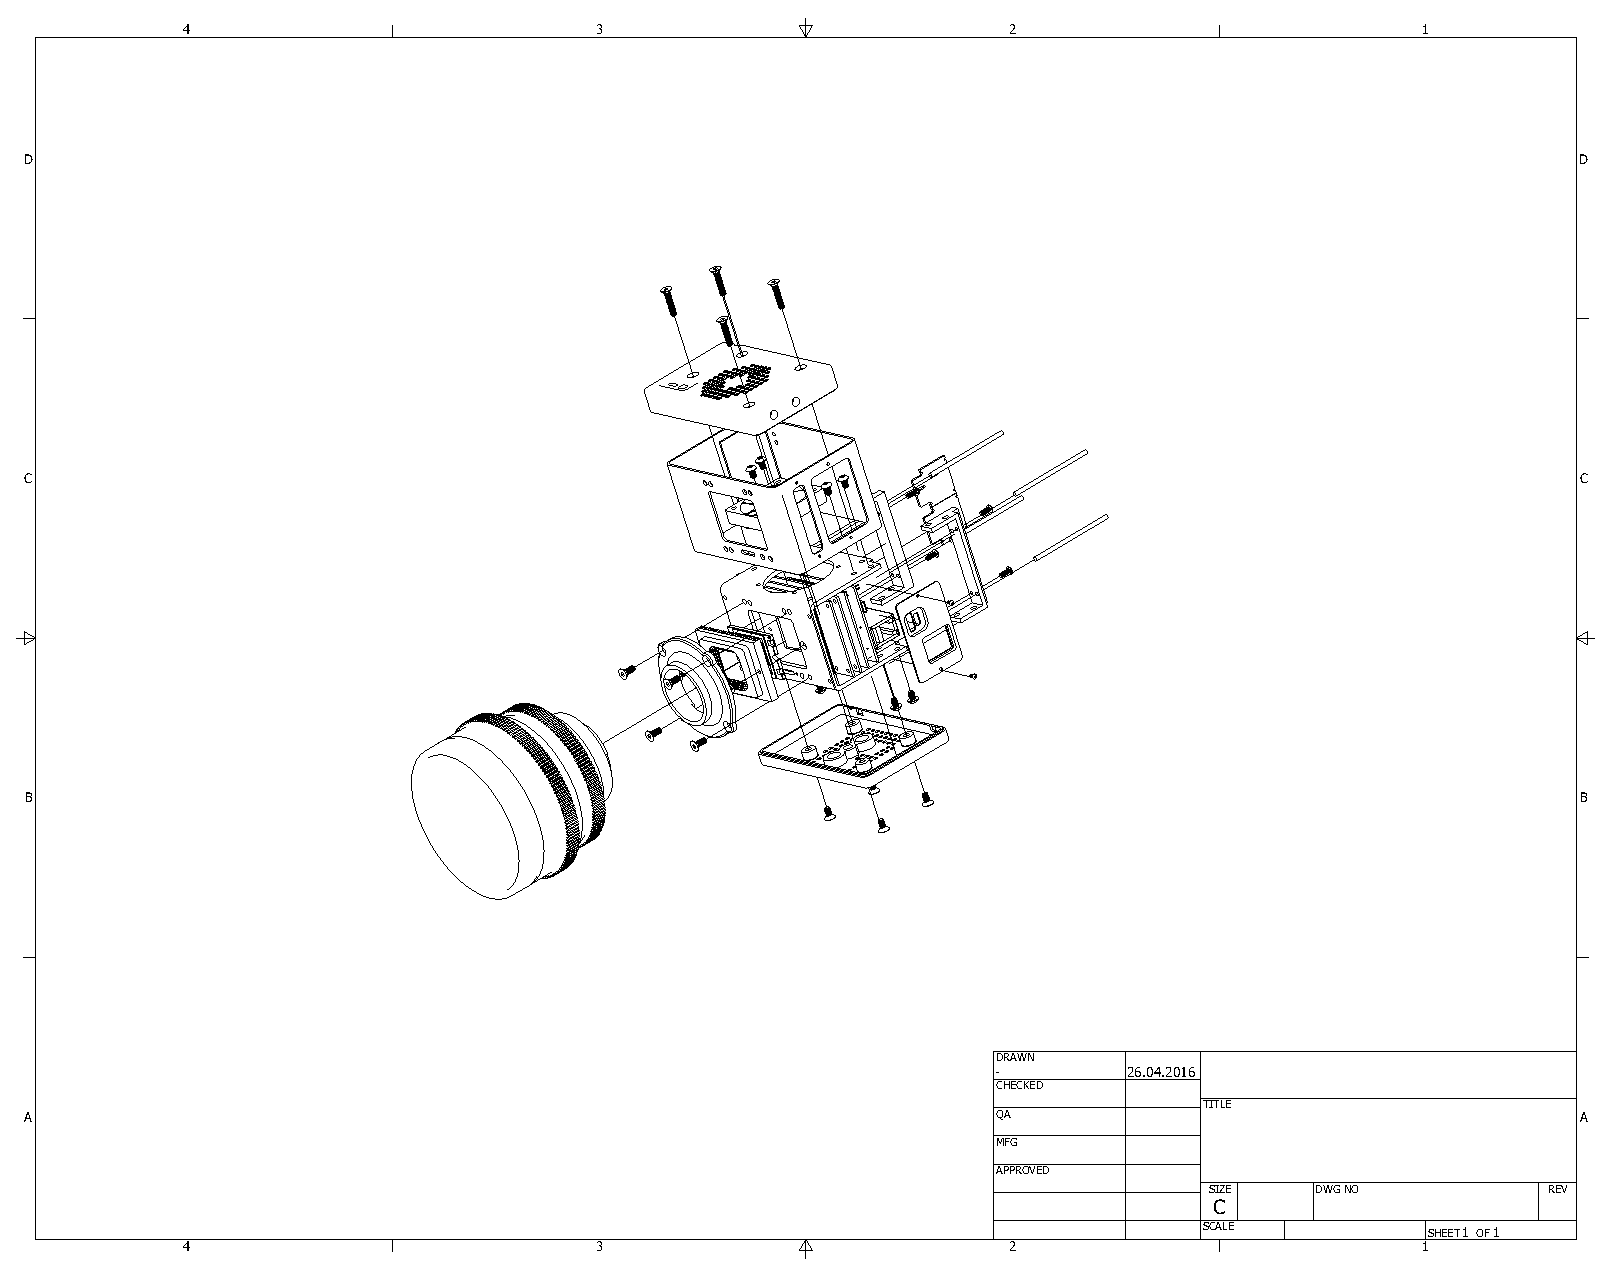
\includegraphics[height=13cm]{images/explosion-full}\\

\textbf{AXIOM Beta User Guide}\\

Permission is granted to copy, distribute and/or modify this document under the terms of the Creative Commons Attribution 4.0 International Public License (CC BY-SA 4.0).\\

Published by apertus° Association.\\


For more information, email team@apertus.org or visit \href{https://apertus.org}{apertus.org}

\end{titlepage}

\tableofcontents

\vspace*{\fill}
\textbf{Note:} In some instances the instructions we have prepared are written in a manor that can be followed by people without a deep technical knowledge. If you are an advanced user please keep this in mind.\\
\\This document has been compiled using LaTeX and its files are stored in the apertus GitHub repository here. If you choose to make any changes to this document please notify a member of the Team so that those changes can be implimented into instances of this guide that are being made available in other locations and formats eg. the project's Wiki page.

\section{General Informaion}


\textbf{Notes on Userspace:} Arch Linux comes with systemd, which has one advantage that the boot process is incredibly fast. Standard tools such as sshd and dhcpcd have been preinstalled.\\

One idea to store camera relevant parameters inside the camera and provide access from most programming languages is to use a database like \href{http://en.wikipedia.org/wiki/Berkeley_DB}{http://en.wikipedia.org/wiki/Berkeley\_DB}


\subsection{AXIOM Beta Connector Overview}
	\subsection{Mountpoints}
	\subsection{Accessories and connected devices}
	

\section{Operating Basics}

\subsection{Prepare your AXIOM Beta for use}

Use a micro-USB cable to connect the camera's MicroZed development board (USB UART) to a computer. The MicroZed board is the backmost, red PCB. (There is another micro-USB socket on the Power Board, but that is the JTAG Interface.)\\

1. Connect the ethernet port on the MicroZed to an ethernet port on your computer. You might have to use an ethernet adapter on newer, smaller machines which come without a native ethernet port.\\ 

2. Connect the AC adapter to the camera's Power Board. (The power cord plugs into an adapter that connects to the Power Board; to power the camera off at a later point, you need not disconnect the adapter from the board but can just unplug the cord from the adapter.)


\subsection{Prepare your computer for use with AXIOM Beta}

\textbf{Overview -} To communicate with your AXIOM Beta camera, you will send it instructions via your computer's command line.\\

In case you have not worked with a shell (console, terminal) much or ever before, we have prepared detailed instructions to help you get you set up. The steps which need to 	be taken to prepare your machine sometimes differ between operating systems, so pick the ones that are applicable to you(r system). \\

Note that dollar signs placed in front of commands are not meant to be typed in but denote 	the command line prompt (a signal indicating the computer is ready for user input). It is used in documentation to differentiate between commands and output resulting from commands. The prompt might look different on your machine (e.g. an angled bracket >) and be preceded by your user name, computer name or the name of the directory which you are currently inside.



\subsubsection{USB to UART Drivers}

For the USB connection to work, you will need drivers for bridging USB to UART (USB to serial). (Under Linux this works out of the box in most 	distributions) for other operating systems they can be 

\hyperlink{https://www.silabs.com/products/development-tools/software/usb-to-uart-bridge-vcp-drivers}{downloaded}
downloaded from e.g. Silicon Labs' website – pick the software provided for your OS and install it. \\

\subsubsection{Serial Console}
\paragraph{Linux Setup}
\paragraph{MAC OSX Setup}
\paragraph{Minicom Configuration}
\subsubsection{Serial connection (via USB)}
\paragraph{Connect using Minicom}\mbox{}\\
Note that you will not be able to use the terminal window you initiate the serial connection in for anything else (it needs to remain open while you access the camera), so it might make sense to open a separate window just for this purpose.

With minicom installed and properly configured, all you need to do is run the following command to start it with the correct settings:

\begin{lstlisting}[language=bash,frame=none,xleftmargin=.25in,belowskip=2em, aboveskip=2em]
$ minicom -8 USB0
\end{lstlisting}

On successful connection, you will be prompted to enter user credentials (which are needed to log into the camera).

If your terminal remains blank except for the minicom welcome screen/information about your connection settings, try pressing enter. If this still does not result in the prompt for user credentials – while testing, we discovered the initial connection with minicom does not always work – disconnect the camera from the power adapter, then reconnect it: in your minicom window you should now see the camera's operating system booting up, followed by the login prompt. (From then on, connecting with minicom should work smoothly and at most require you to press enter to make the login prompt appear.)

\paragraph{Connect using Screen}
\paragraph{Disconnect}
\subsubsection{Ethernet connection (using SSH)}
\paragraph{SSH Keys how-to for Linux and Mac}
\subparagraph{Storage location/Find existing keys}
\subparagraph{SSH key creation}
\paragraph{Get or set IP address}
\paragraph{IP address check}
\paragraph{Set IP address}
\paragraph{Establish a connection via key}
\paragraph{Password-based authentication}
\subsubsection{Start the camera}
\subsubsection{WiFi access point setup}
\section{Writing Images}

For writing uncompressed full resolution full bitdepth raw images the AXIOM Beta uses a software called cmv_snap3.\\

It is located in the /root/ directory and writes the images data directly to STDOUT.\\

cmv_snap3 writes images in the \href{https://wiki.apertus.org/index.php/RAW12}{RAW12} format. Writing one image takes a few seconds depending on where the image is written to so this method is not viable for recording video footage other than timelapse. 




\subsection{Capture Still Images}
\subsubsection{Parameters}

The following parameters are available:

\begin{lstlisting}[language=bash,morekeywords=$,keywordstyle=\bfseries,frame=none,xleftmargin=.25in,belowskip=2em, aboveskip=2em]
    ./cmv_snap3 -h
    This is ./cmv_snap3 V1.10
    options are:
    -h        print this help message
    -8        output 8 bit per pixel
    -2        output 12 bit per pixel
    -d        dump buffer memory
    -b        enable black columns
    -p        prime buffer memory
    -r        dump sensor registers
    -t        enable cmv test pattern
    -z        produce no data output
    -e <exp>  exposure times
    -v <exp>  exposure voltages
    -s <num>  shift values by <num>
    -S <val>  writer byte strobe
    -R <fil>  load sensor registers
\end{lstlisting} 

\textbf{Examples}\\

Images can be written directly to the cameras internal micro SD card like this (10 milliseconds exposure time, 16bit):

\begin{lstlisting}[language=bash,morekeywords=$,keywordstyle=\bfseries,frame=none,xleftmargin=.25in,belowskip=2em, aboveskip=2em]
./cmv_snap3 -e 10ms > image.raw16
\end{lstlisting} 

Write image plus metadata (sensor configuration) to cameras internal micro SD card (20 milliseconds exposure time, 12bit): 

\begin{lstlisting}[language=bash,morekeywords=$,keywordstyle=\bfseries,frame=none,xleftmargin=.25in,belowskip=2em, aboveskip=2em]
./cmv_snap3 -2 -r -e 20ms > image.raw12
\end{lstlisting} 

You can also use cmv_snap3 to change to exposure time (to 5 milliseconds in this example) without actually capturing an image, for the that -z parameter is used to not produce any data output: 

\begin{lstlisting}[language=bash,morekeywords=$,keywordstyle=\bfseries,frame=none,xleftmargin=.25in,belowskip=2em, aboveskip=2em]
./cmv_snap3 -z -e 5ms
\end{lstlisting} 

That cmv_snap3 writes data to STDOUT makes it very versatile, we can for example capture images from and to a remote Linux machine connected to the Beta via Ethernet easily (lets assume the AXIOM Betas camera IP is set up as: 192.168.0.9 - SSH access has to be set up for this to work with a keypair) 

\begin{lstlisting}[language=bash,morekeywords=$,keywordstyle=\bfseries,frame=none,xleftmargin=.25in,belowskip=2em, aboveskip=2em]
ssh root@192.168.0.9 "./cmv_snap3 -2 -r -e 10ms" > snap.raw12
\end{lstlisting} 

To pipe the data into a file and display it at the same time with imagemagick on a remote machine: 

\begin{lstlisting}[language=bash,morekeywords=$,keywordstyle=\bfseries,frame=none,xleftmargin=.25in,belowskip=2em, aboveskip=2em]
    ssh root@192.168.0.9 "./cmv_snap3 -2 -r -e 10ms" | tee snap.raw12 | display -size 4096x3072 -depth 12 gray:-
\end{lstlisting} 

Use imagemagick to convert raw12 file into a color preview image: 

\begin{lstlisting}[language=bash,morekeywords=$,keywordstyle=\bfseries,frame=none,xleftmargin=.25in,belowskip=2em, aboveskip=2em]
cat test.raw12 | convert \( -size 4096x3072 -depth 12 gray:- \) \( -clone 0 -crop -1-1 \) \( -clone 0 -crop -1+0 \) \( -clone 0 -crop +0-1 \) -sample 2048x1536 \( -clone 2,3 -average \) -delete 2,3 -swap 0,1 +swap -combine test_color.png
\end{lstlisting} 


With raw2dng compiled inside the camera you can capture images directly to DNG, without saving the raw12: 


\begin{lstlisting}[language=bash,morekeywords=$,keywordstyle=\bfseries,frame=none,xleftmargin=.25in,belowskip=2em, aboveskip=2em]
./cmv_snap3 -2 -b -r -e 10ms | raw2dng snap.DNG
\end{lstlisting} 


\textbf{Note:} Supplying exposure time as parameter is required otherwise cmv_snap3 will not capture an image. The exposure time can be supplied in "s" (seconds), "ms" (milliseconds), "us" (microseconds) and "ns" (nanoseconds). Decimal values also work (eg. "15.5ms"). 


\subsection{Image Overlays}

This section covers the mimg version 1.8 (see \href{https://github.com/apertus-open-source-cinema/beta-software/tree/master/mimg}{GitHub repo}), not the previous 1.6. 

AXIOM Beta features a full HD framebuffer that can be altered from the Linux userspace and is automatically "mixed" with the real time video from the image sensor on HDMI outputs.\\

The overlay could also be used to draw live histograms/scopes/HUD or menus.\\

The overlay in more recent firmware revisions supports alpha channel transparency. \\


\subsubsection{Internals}


The raw memory image is saved the following way: <ch0/12bit><ch1/12bit><ch2/12bit><ch3/12bit><overlay/16bit> \\

This means that for every 4 sensels there is only one overlay pixel. Meaning, while the CMV12000 image sensor is 4Kx3K the overlay is Full HD (1080p). 


\subsubsection{Prepare Images}

Convert 24bit PNG (1920x1080 pixels) with transparency to AXIOM Beta raw format: 

\begin{lstlisting}[language=bash,morekeywords=$,keywordstyle=\bfseries,frame=none,xleftmargin=.25in,belowskip=2em, aboveskip=2em]
convert input.png rgba:output.rgb
\end{lstlisting}

\textbf{Note :} This image format is different from \href{https://wiki.apertus.org/index.php/RAW12}{RAW12}.


\subsubsection{mimg}

mimg is software running on the camera that's used to load/alter anything related to overlays or test images.\\

Source code is available on \href{https://github.com/apertus-open-source-cinema/beta-software/tree/master/mimg}{GitHub}.

\begin{lstlisting}[language=bash,morekeywords=$,keywordstyle=\bfseries,frame=none,xleftmargin=.25in,belowskip=2em, aboveskip=2em]
    This is ./mimg V1.8
    options are:
    -h        print this help message
    -a        load all buffers
    -o        load as overlay
    -O        load as color overlay
    -r        load raw data
    -w        use word sized data
    -D <val>  image color depth
    -W <val>  image width
    -H <val>  image height
    -P <val>  uniform pixel color
    -T <val>  load test pattern
    -B <val>  memory mapping base
    -S <val>  memory mapping size
    -A <val>  memory mapping address
\end{lstlisting} 

\textbf{Examples:}\\


Clear overlay: 

\begin{lstlisting}[language=bash,morekeywords=$,keywordstyle=\bfseries,frame=none,xleftmargin=.25in,belowskip=2em, aboveskip=2em]
./mimg -a -o -P 0
\end{lstlisting} 


Load monochrome overlay: 

\begin{lstlisting}[language=bash,morekeywords=$,keywordstyle=\bfseries,frame=none,xleftmargin=.25in,belowskip=2em, aboveskip=2em]
./mimg -o -a file.raw
\end{lstlisting} 


Load color overlay: 

\begin{lstlisting}[language=bash,morekeywords=$,keywordstyle=\bfseries,frame=none,xleftmargin=.25in,belowskip=2em, aboveskip=2em]
./mimg -O -a file.raw
\end{lstlisting} 


Enable overlay: 

\begin{lstlisting}[language=bash,morekeywords=$,keywordstyle=\bfseries,frame=none,xleftmargin=.25in,belowskip=2em, aboveskip=2em]
gen_reg 11 0x0104F000
\end{lstlisting} 


Disable overlay: 

\begin{lstlisting}[language=bash,morekeywords=$,keywordstyle=\bfseries,frame=none,xleftmargin=.25in,belowskip=2em, aboveskip=2em]
gen_reg 11 0x0004F000
\end{lstlisting} 


\textbf{Old overlays}:\\

Overlays for mimg 1.6 are not compatible anymore. You can use

\begin{lstlisting}[language=bash,morekeywords=$,keywordstyle=\bfseries,frame=none,xleftmargin=.25in,belowskip=2em, aboveskip=2em]
convert -size 1920x1080 -depth 6 rgba:overlay_04.rgb overlay_04.png
\end{lstlisting} 

... to convert them to PNG before continuing with the preparation above. 
\section{Changing Camera Parameters}

Some itro text required\\

\subsection{Setting CMV12000 sensor registers}

\textbf{cmv\_reg}

Get and Set CMV12000 image sensor registers (CMV12000 sports 128x16 Bit registers).\\

Details for the sensor datasheet are on GitHub under \href{https://github.com/apertus-open-source-cinema/beta-hardware/tree/master/Datasheets}{Datasheets}\\

\textbf{Examples:}\\

Read register 115 (which contains the analog gain settings): 

\begin{lstlisting}[language=bash,morekeywords=$,keywordstyle=\bfseries,frame=none,xleftmargin=.25in,belowskip=2em, aboveskip=2em]
cmv_reg 115
\end{lstlisting} 

Return value:

\begin{lstlisting}[language=bash,morekeywords=$,keywordstyle=\bfseries,frame=none,xleftmargin=.25in,belowskip=2em, aboveskip=2em]
0x00
\end{lstlisting} 

Means we are currently operating at analog gain x1 = unity gain\\


Set register 115 to gain x2: 

\begin{lstlisting}[language=bash,morekeywords=$,keywordstyle=\bfseries,frame=none,xleftmargin=.25in,belowskip=2em, aboveskip=2em]
cmv_reg 115 1
\end{lstlisting}



\subsection{Setting Exposure Time}

To set the exposure time use the cmv\_snap3 tool with -z parameter (this will tell the software to not save the image): 

\begin{lstlisting}[language=bash,morekeywords=$,keywordstyle=\bfseries,frame=none,xleftmargin=.25in,belowskip=2em, aboveskip=2em]
./cmv_snap3 -e 9.2ms -z
\end{lstlisting}

\textbf{Note:} The exposure time can be supplied in "s" (seconds), "ms" (milliseconds), "us" (microseconds) and "ns" (nanoseconds). Decimal values also work (eg. "15.5ms"). 



\subsection{Setting gain value}

\textbf{set\_gain.sh}\\

Set gain and related settings (ADC range and offsets). 

\begin{lstlisting}[language=bash,morekeywords=$,keywordstyle=\bfseries,frame=none,xleftmargin=.25in,belowskip=2em]
    ./set_gain.sh 1 
    ./set_gain.sh 2
    ./set_gain.sh 3/3 # almost the same as gain 1
    ./set_gain.sh 3
    ./set_gain.sh 4
\end{lstlisting}



\subsection{Setting Gamma Values}

\textbf{gamma\_conf.sh}\\

Set the gamma value: 

\begin{lstlisting}[language=bash,morekeywords=$,keywordstyle=\bfseries,frame=none,xleftmargin=.25in,belowskip=2em]
    ./gamma_conf.sh 0.4
    ./gamma_conf.sh 0.9
    ./gamma_conf.sh 1
    ./gamma_conf.sh 2
\end{lstlisting}


\section{Image metadata}
The RAW12 is designed to contain native raw image sensor data for image written by the AXIOM Beta and can optionally also contain an image sensor registers dump (128 x 16bit, big endian) appened at the end of file.  

The \importantKeyword{-r} command indicates to include the sensor registers when capturing an image (See Section \ref{sec:capture_still_images}):
\consoleCommand{./cmv\_snap3 -r -e 10ms > image.raw12}

Show metadata from a RAW12 file (without converting it):

\consoleCommand{raw2dng file.raw12 --dump-regs}

or, with \href{https://github.com/apertus-open-source-cinema/misc-tools-utilities/tree/master/cmv12000-metadata-reader}{metadatareader}:

\consoleCommand{cat image.raw12 | dd bs=256 skip=73728 | ./metadatareader}

Details about the meaning of all image sensor registers can be found in the image sensor  \href{https://github.com/apertus-open-source-cinema/beta-hardware/tree/master/Datasheets}{datasheet}. 

\subsection{Image Histogram Data}

To read and output histogram data from the Betas live image a tool called \importantKeyword{cmv\_hist3} is available inside the AXIOM Beta.

\begin{lstlisting}[language=bash,morekeywords=$,keywordstyle=\bfseries,frame=none,xleftmargin=.25in,belowskip=2em]
./cmv\_hist3 -h                                                   
This is ./cmv_hist3 V1.4                                                        
options are:                                                                    
-h        print this help message                                               
-s        acquire snapshot                                                      
-b <num>  number of bins                                                        
-d <num>  decimation factor                                                     
-r <num>  number of rows                                                        
-C <prc>  center sample area                                                    
-B <val>  register mapping base                                                 
-S <val>  register mapping size
\end{lstlisting}

The output in 12 bit mode (default) are values in 4096 lines and 4 columns (R, G, B, GB channels) 
\section{Output}

Intro text required




\subsection{HDMI}

HDMI is a two-way communication protocol and supports many different formats/frequencies/specs. Many monitors/recorders only support a subset of these formats and expect signals to conform to certain values. These values are not documented publicly so we are currently in the process of debugging device compatibility one by one. The good thing is that it's a pure software thing and we can add support and test compatibility with additional devices as time progresses.\\

In general we discovered that monitors are more flexible when it comes to HDMI (TMDS) freqencies as they just "tune" into (sync to) the provided clock/data rate. Recorders expect signals to be in a much stricter/narrower range and will not work (show "no signal") if there is a minor deviation. 

Watch this 33C3 talk by Tim Ansell about \href{https://media.ccc.de/v/33c3-8057-dissecting_hdmi}{Dissecting HDMI} to get insight into how HDMI works.




\subsubsection{External HDMI Recording}

Settings for VSync, HSync, etc. inside the AXIOM Beta can be found in: 

\consolecommand{/root/gen\_init.sh}

For example the Atomos SHOGUN was found to work with these HDMI parameters:  

\begin{lstlisting}[breaklines=true, breakatwhitespace=true]
scn\_reg  0 2200             # total\_w
scn\_reg  1 1125             # total\_h
scn\_reg  2   60             # total\_f

scn\_reg  4  262             # hdisp\_s
scn\_reg  5 2182             # hdisp\_e
scn\_reg  6   45             # vdisp\_s
scn\_reg  7 1125             # vdisp\_e

scn\_reg  8    0             # hsync\_s
scn\_reg  9 2100             # hsync\_e
scn\_reg 10    4             # vsync\_s
scn\_reg 11    9             # vsync\_e

scn\_reg 32  252             # pream\_s
scn\_reg 33  260             # guard\_s
scn\_reg 34  294             # terc4\_e
scn\_reg 35  296             # guard\_e
\end{lstlisting}

Currently it is not possible to alter TMDS and Clock frequencies from the userspace (requires new FPGA bitstream).\\

For the firmware there are two modes available, the 30Hz and 60Hz variant. You can switch between them quite easily.\\

cmv\_hdmi3.bit is the FPGA bitstream loaded for the HDMI interface. We use symlinks to switch this file easily.\\

Before doing this, don't forget to check if the files (cmv\_hdmi3\_60.bit or cmv\_hdmi3\_30.bit) really exist in the /root folder.\\

The output is always in 8bpc RGB color space without subsampling (4:4:4). Not all capture devices can manage this.\\

Other modes like YCrCb, etc. are currently not supported.\\ 




\paragraph{Devices Confirmed Working}

Atomos Shogun - AXIOM Beta supports up to 1080p60 
Atomos Ninja - AXIOM Beta supports up to 1080p30
Blackmagic Video Assist and Video Assist 4K - AXIOM Beta supports up to 1080p60\\

\textbf{Blackmagic Video Assist and Video Assist 4K}

\begin{center}
	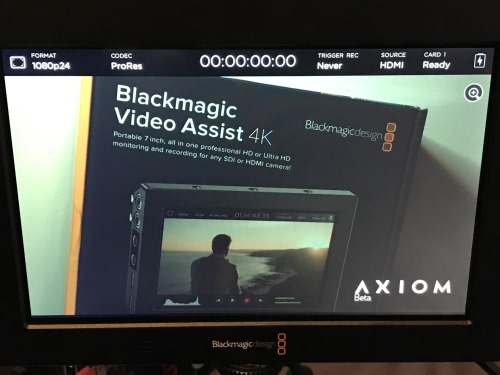
\includegraphics[height=8cm]{images/AxiomBetaBMVA4K}\\
\end{center}

Changes for Blackmagic Video Assist and Video Assist 4K, tested on firmware 2.3.1:\\

\textbf{edit setup.sh}\\

Add: 

\consolecommand{./gen\_init.sh 1080p60BMVA}

comment out any other ./gen\_init.sh entries. 

\textbf{edit gen\_init.sh}

\consolecommand{./gen\_init.sh 1080p60BMVA}

\textbf{edit gen\_init.sh}

Replace:

\consolecommand{SHOGUN)}

With:

\consolecommand{SHOGUN|1080p60BMVA|1080p30BMVA)}

Add the section below:

\consolecommand{  
	1080p50BMVA|1080p25BMVA)^^J
	scn\_reg  0 2640	# total\_w^^J
	scn\_reg  1 1125    # total\_h^^J
	scn\_reg  2   60    # total\_f^^J
	^^J
	scn\_reg  4  262    # hdisp\_s^^J
	scn\_reg  5 2182    # hdisp\_e^^J
	scn\_reg  6   45    # vdisp\_s^^J
	scn\_reg  7 1125    # vdisp\_e^^J
	^^J
	scn\_reg  8    0    # hsync\_s^^J
	scn\_reg  9 2100    # hsync\_e^^J
	scn\_reg 10    4    # vsync\_s^^J
	scn\_reg 11    9    # vsync\_e^^J
	^^J
	scn\_reg 32  252	# pream\_s^^J
	scn\_reg 33  260    # guard\_s^^J
	scn\_reg 34  294    # terc4\_e^^J
	scn\_reg 35  296    # guard\_e^^J
	;;
	^^J
	^^J
	1080p24BMVA)^^J
	scn\_reg  0 2750    # total\_w^^J
	scn\_reg  1 1125    # total\_h^^J
	scn\_reg  2   60    # total\_f^^J
	^^J
	scn\_reg  4  262    # hdisp\_s^^J
	scn\_reg  5 2182    # hdisp\_e^^J
	scn\_reg  6   45    # vdisp\_s^^J
	scn\_reg  7 1125    # vdisp\_e^^J
	^^J
	scn\_reg  8    0    # hsync\_s^^J
	scn\_reg  9 2100    # hsync\_e^^J
	scn\_reg 10    4    # vsync\_s^^J
	scn\_reg 11    9    # vsync\_e^^J
	^^J
	scn\_reg 32  252    # pream\_s^^J
	scn\_reg 33  260    # guard\_s^^J
	scn\_reg 34  294    # terc4\_e^^J
	scn\_reg 35  296    # guard\_e^^J
	;;
}




\subsubsection{Experimental UHD Raw Recording}

\textbf{Note:} This experimental raw mode works only in 1080p60 (A+B Frames) and is only tested with the Atomos Shogun currently. \\

To measure the required compensations with a different recorder see \textbf{Raw processing recorder benchmarking}\\

This mode requires darkframes which are created in the course of a camera Factory Calibration. Early Betas are not calibrated yet - this step needs to be completed by the user. See \textbf{Factory Calibration}.\\




\paragraph{Enable raw recording mode}\mbox{}\\

Input:

\consolecommand{\./hdmi\_rectest.sh}

Inside that script the following command is worth noting:\\

Enable experimental raw mode: 

\consolecommand{scn\_reg 31 0x0A01}

Disable experimental raw mode: 

\consolecommand{scn\_reg 31 0x0001}

If you get an error report like this: 

\consolecommand{    Traceback (most recent call last):
	File "rcn\_darkframe\.py", line 17, in <module>
	import png
	ImportError: No module named 'png'}

Make sure the Beta is connected to the Internet via Ethernet and run:     

\consolecommand{pip install pypng}




\paragraph{Processing}

Postprocessing software to recover the raw information (DNG sequences) is on github in \href{https://github.com/apertus-open-source-cinema/misc-tools-utilities/tree/master/raw-via-hdmi}{RAW via HDMI}

Required packages: ffmpeg build-essentials

Mac requirements for compiling: gcc4.9(via homebrew): 

\consolecommand{brew install homebrew/versions/gcc49}

Also install ffmpeg\\

To do all the raw processing in one single command (after ffmpeg codec copy processing): 

\consolecommand{\./hdmi4k INPUT\.MOV - | \./raw2dng --fixrnt --pgm --black=120 frame\%05d\.dng}
	
	
	
	
\subsubsection{Experimental UHD Raw Recording}

\textbf{Note:} This experimental raw mode works only in 1080p60 (A+B Frames) and is only tested with the Atomos Shogun currently. \\

To measure the required compensations with a different recorder see \textbf{Raw processing recorder benchmarking}\\

This mode requires darkframes which are created in the course of a camera Factory Calibration. Early Betas are not calibrated yet - this step needs to be completed by the user. See \textbf{Factory Calibration}.\\




\paragraph{Enable raw recording mode}\mbox{}\\

Input:

\consolecommand{\./hdmi\_rectest.sh}

Inside that script the following command is worth noting:\\

Enable experimental raw mode: 

\consolecommand{scn\_reg 31 0x0A01}

Disable experimental raw mode: 

\consolecommand{scn\_reg 31 0x0001}

If you get an error report like this: 

\consolecommand{    Traceback (most recent call last):
	File "rcn\_darkframe\.py", line 17, in <module>
	import png
	ImportError: No module named 'png'}

Make sure the Beta is connected to the Internet via Ethernet and run:     

\consolecommand{pip install pypng}




\subparagraph{Raw processing recorder benchmarking}
	
We can analyze footage recorded by the 3rd party recorder but we would need the following:\\
	
- Make sure your Beta is running in experimental 4k raw mode (1080p60 with A+B frames)\\
- Short HDMI captured clip from the 3rd party recorder\\
- Raw12 still image captured during the HDMI recording\\
	
This kind of script is helpful to execute during HDMI recording: 
	
\consolecommand{
	# stop HDMI stream:^^J
	fil\_reg 15 0^^J
	^^J
	# capture image^^J
	\./cmv\_snap3 -r -2 -e 10ms > image\.raw12^^J
	^^J
	# start HDMI stream:^^J
	fil\_reg 15 0x01000100
}

Taking a snapshot during HDMI recording with the above script will pause the HDMI stream for a few seconds, where it will alternate between two frames. These two frames will be from the same raw data as image.raw12, so they contain all that's needed to figure out what kind of processing the HDMI recorder applies to the image, and how to undo it in order to recover the raw data.\\
	
Ideally, the scene should contain fine details (such as tissue, fine print) and rich colors. A color chart (which usually contains some fine print as well) is a very good choice. \\
	
... and finally we'd need:\\
	
- HDMI captured 1-minute clip with dark frames (lens cap on camera, black cloth covering camera in a dark room)
	
	
	
	
\subparagraph{Factory Calibration}
	
Create a variable containing your Betas IP for easy access:
\consolecommand{export BETA=192.168.1.101}
	
\textbf{Preperations:}\\
	
Install on your AXIOM Beta: 
	
\consolecommand{pacman -S python-numpy}
	
Install the following packages on your PC: 
	
\consolecommand{dcraw octave}
	
For Ubuntu this would look like: 
	
\consolecommand{sudo apt-get install dcraw octave}
	
\textbf{Step 1: Check range of the input signal}\\
	
On the Beta set gain to x1 by running: 
	
\consolecommand{./set\_gain.sh 1}
	
Download this Octave file to your PC into your current work directory: 
	
\begin{lstlisting}[breaklines=true, breakatwhitespace=true]
wget https://raw.githubusercontent.com/apertus-open-source-cinema/misc-tools-utilities/master/darkframes/read\_raw.m
\end{lstlisting}
	
Capture an overexposed image with the Beta and check the levels:\\ 
	
\begin{lstlisting}[breaklines=true, breakatwhitespace=true]
	ssh root@$BETA "./cmv\_snap3 -2 -b -r -e 100ms" > snap.raw12
	./raw2dng snap.raw12 --totally-raw
	octave
	octave:1> a = read\_raw('snap.DNG')
	octave:2> prctile(a(:), [0.1 1 50 99 99.9])
\end{lstlisting}

If everything worked you will get a wall of numbers now.\\ 
	
Lower numbers should be around 50...300 (certainly not zero). Higher numbers should be around 4000, but not 4095.\\
	
Repeat for gains 2, 3, 4.\\
	
Put this in startup script ie: \importantKeyword{kick\_manual.sh} (The systemd service cmv12k is autostarted when boot on and calls the \importantKeyword{kick.sh} and \importantKeyword{halt.sh} scripts on startup and shutdown respectively and those scripts in turn call the \importantKeyword{kick\_manual.sh} and \importantKeyword{halt\_manual.sh} which also should be used when the cmv12k service is disabled for whatever reason) : 
	
\consolecommand{./set\_gain.sh 1}   
	
\textbf{Step 2: RCN calibration}\\
	
Make sure you have \href{https://github.com/apertus-open-source-cinema/beta-software/tree/master/beta-scripts}{these scripts} already in your Beta's /root/ directly.\\
	
Clear the old RCN values: 
	
\consolecommand{
	ssh root@\$BETA "./rcn\_clear.py"
}
 
	
Now you need to make sure that your Beta is not capturing any light (ideally not a single photon should hit the sensor) :\\
	
1. lose the lens aperture as far as possible\\
2. Attach lens cap\\
3. Put black lens bag over Beta\\
4. Turn off all lights in the room - do this at night or in a completely dark room \\
	
Take 64 dark frames at 10ms, gain x1. 
	
\begin{lstlisting}[breaklines=true, breakatwhitespace=true]
	./set\_gain.sh 1
	fil_reg 15 0 # disable HDMI stream
	for i in `seq 1 64`; do
	ssh root@$BETA "./cmv\_snap3 -2 -b -r -e 10ms" > dark-x1-10ms-$i.raw12 
	done 
	fil_reg 15 0x01000100  # enable HDMI stream
\end{lstlisting}
	
Compute a temporary dark frame for RCN calibration: 
	
\consolecommand{raw2dng --swap-lines --no-blackcol --calc-darkframe dark-x1-10ms-*.raw12} 
	
This should process quite quickly and output something like the following at the end: 
	
\consolecommand{    Averaged 64 frames exposed from 12.00 to 12.00 ms.
	Could not compute dark current.
	Please use different exposures, e.g. from 1 to 50 ms.
	Dark offset : 0.00
	Writing darkframe-x1.pgm...
	Done.} 

Rename and upload darkframe to your Beta:  

\begin{lstlisting}[breaklines=true, breakatwhitespace=true]
mv darkframe-x1.pgm darkframe-rcn.pgm
scp darkframe-rcn.pgm root@$BETA:/root/
\end{lstlisting} 

Set the RCN values: 

\begin{lstlisting}[breaklines=true, breakatwhitespace=true]
ssh root@$BETA "./rcn\_darkframe.py darkframe-rcn.pgm"
\end{lstlisting} 

Put this in startup script ie : \importantKeyword{kick\_manual.sh } :

\begin{lstlisting}[breaklines=true, breakatwhitespace=true]
./rcn\_darkframe.py darkframe-rcn.pgm 
\end{lstlisting} 

If you get an error report like this: 

\begin{lstlisting}[breaklines=true, breakatwhitespace=true]
Traceback (most recent call last):
File "rcn\_darkframe.py", line 17, in <module>
import png
ImportError: No module named 'png'
\end{lstlisting} 

Make sure the Beta is connected to the Internet via Ethernet and run: 

\consolecommand{pip install pypng}

and then run the python script again.\\

\textbf{Validation}\\

\textbf{Method 1:}\\
	
Put a lens cap on the camera and check the image on a HDMI monitor.\\

In the camera set the matrix gains to: 

\consolecommand{./mat4\_conf.sh  20 0 0 0  0 10 10 0  0 10 10 0  0 0 0 10  0 0 0 0}

run:

\consolecommand{./rcn\_clear.py}

The static noise profile should be visible.\\

run: 

\consolecommand{./rcn\_darkframe.py darkframe-rcn.pgm }

The static noise profile should be gone. You will still see dynamic row noise (horizontal lines flickering) - thats expected.\\


\textbf{Method 2:}\\

This method is now entirely automated with running one script inside the camera: \href{https://github.com/apertus-open-source-cinema/beta-software/blob/master/beta-scripts/rcn_validation.sh}{https://github.com/apertus-open-source-cinema/beta-software/blob/master/beta-scripts/rcn\_validation.sh}\\

Capture one darkframe without compensations: \\

\begin{lstlisting}[breaklines=true, breakatwhitespace=true]
ssh root@$BETA "./rcn\_clear.py"
ssh root@$BETA "./cmv\_snap3 -2 -b -r -e 10ms" > dark-check-1.raw12
\end{lstlisting} 

Capture one darkframe with compensations: \\

\begin{lstlisting}[breaklines=true, breakatwhitespace=true]
ssh root@$BETA "./rcn\_darkframe.py darkframe-rcn.pgm"
ssh root@$BETA "./cmv\_snap3 -2 -b -r -e 10ms" > dark-check-2.raw12 
\end{lstlisting} 

Then use \importantKeyword{raw2dng} to analyze the differences: \\

\begin{lstlisting}[breaklines=true, breakatwhitespace=true]
raw2dng --no-darkframe --check-darkframe dark-check-1.raw12
raw2dng --no-darkframe --check-darkframe dark-check-2.raw12
\end{lstlisting} 

With the compensated snapshot the column noise should disappear, and only row noise left should be dynamic (not static). Visual inspection: the dark frame should have only horizontal lines, not vertical ones.\\

Sample output:\\ 

\begin{lstlisting}[breaklines=true, breakatwhitespace=true]
Average     : 127.36               # about 128, OK
Pixel noise : 5.44                 # this one is a bit high because we only corrected row and column offsets (it's OK)
Row noise   : 2.30 (42.2%)         # this one should be only dynamic row noise - see Method 3 below.
Col noise   : 0.20 (3.8%)          # this one is very small, that's what we need to check here}
\end{lstlisting} 


\textbf{Method 3:}\\

Capture 2 frames: \\

\begin{lstlisting}[breaklines=true, breakatwhitespace=true]
ssh root@$BETA "./cmv\_snap3 -2 -b -r -e 10ms" > dark-check-1.raw12 
ssh root@$BETA "./cmv\_snap3 -2 -b -r -e 10ms" > dark-check-2.raw12 
\end{lstlisting} 

Convert the two darkframes with raw2dng: \\

\consolecommand{raw2dng dark-check-*}

Make sure you have the required octave function file in place:\\ 

\begin{lstlisting}[breaklines=true, breakatwhitespace=true]
wget https://raw.githubusercontent.com/apertus-open-source-cinema/misc-tools-utilities/master/darkframes/read_raw.m
\end{lstlisting} 

Also you need to install the octave "signal" and "control" packages from \href{http://octave.sourceforge.net/packages.php}{http://octave.sourceforge.net/packages.php} then, inside octave, run to install:\\

\consolecommand{pkg install package\_name}

To check whether the entire row noise is dynamic, load the two raw images in octave and check the autocorrelation between the two row noise samples: \\

\begin{lstlisting}[breaklines=true, breakatwhitespace=true]
pkg load signal
a = read\_raw('dark-check-1.DNG');
b = read\_raw('dark-check-2.DNG');
ra = mean(a'); ra = ra - mean(ra);
rb = mean(b'); rb = rb - mean(rb);
xcov(ra, rb, 0, 'coeff')
\end{lstlisting} 

Result should be very small (about 0.1 or lower). When running this check on two uncalibrated dark frames, you will get around 0.8 - 0.9.\\

\textbf{Step 3: Dark frame calibration}\\

Make sure the RCN calibration from previous steps is in place before continueing here.\\

Take dark frames at various exposure times and gains.\\

\begin{lstlisting}[breaklines=true, breakatwhitespace=true]
for i in 1 2 3 4; do
for e in `seq 1 100`; do
for g in 1 2 3 4; do
ssh root@$BETA "./set\_gain.sh $g"
ssh root@$BETA "./cmv\_snap3 -2 -b -r -e ${e}ms" > dark-x${g}-${e}ms-$i.raw12
done
done
done
\end{lstlisting} 

Compute dark frames for each gain: \\

\consolecommand{    raw2dng --swap-lines --calc-dcnuframe dark-x1-*.raw12
	raw2dng --swap-lines --calc-dcnuframe dark-x2-*.raw12
	raw2dng --swap-lines --calc-dcnuframe dark-x3-*.raw12
	raw2dng --swap-lines --calc-dcnuframe dark-x4-*.raw12
}

Save the following files (N=1..4): 
	
\consolecommand{
	darkframe-xN.pgm
	dcnuframe-xN.pgm
}

These files should be used in postprocessing. Place them in the directory where you capture raw12 files, so raw2dng will use them.\\

\textbf{Validation}\\ 

On the same dark frames, or - even better - on a new set of dark frames, run: 

\consolecommand{raw2dng --swap-lines --check-darkframe dark*.raw12 > dark-check.log}

Upload the log for detailed analysis.\\

Typical good values are:\\

average value: close to 128\\

pixel noise: about 3 or 4 (may increase at longer exposure times)\\

row noise and column noise: similar to Step 2\\

\textbf{Step 4: Color profiling}\\

Set gain x1:\\

\begin{lstlisting}[breaklines=true, breakatwhitespace=true]
ssh root@$BETA "./set_gain.sh 1"
\end{lstlisting} 

Take a picture of the IT8 chart, correctly exposed.\\

Edit the coordinates and the raw file name in \importantKeyword{calib\_argyll.sh} ( \href{https://github.com/apertus-open-source-cinema/misc-tools-utilities/blob/master/color-calibration/calib_argyll.sh}{https://github.com/apertus-open-source-cinema/misc-tools-utilities/blob/master/color-calibration/calib\_argyll.sh} ). \\

\begin{lstlisting}[breaklines=true, breakatwhitespace=true]
ssh root@$BETA "./cmv\_snap3 -2 -b -r -e 10ms" > it8chart.raw12
./calib\_argyll.sh IT8
\end{lstlisting}

Save the following files:\\

- ICC profile (*.icc)\\
- OCIO configuration (copy/paste from terminal) + LUT file (*.spi1d)\\ 

\textbf{Validation}\\

Render the IT8 chart in Blender, using the OCIO configuration.\\

Same with the ICC profile (Adobe? RawTherapee? What apps support ICC?)\\

(todo: detailed steps)\\

\textbf{Step 5: HDMI dark frames }\\

Record a 1-minute clip with lens cap on.\\

Average odd and even frames.\\

(todo: polish and upload the averaging script)\\

(todo: check if the HDMI dark frames can be computed from regular dark frames)\\

Results: darkframe-hdmi-A.ppm and darkframe-hdmi-B.ppm.\\

\textbf{Step 6: HDMI filters for raw recovery }\\

This calibration is for the recorder, not for the camera. It's for recovering the original raw data from the HDMI, so it has nothing to do with sensor profiling and such.\\

Record some scene with high detail AND rich colors.\\

Take a raw12 snapshot in the middle of recording. The HDMI stream will pause for a few seconds.\\

Upload two frames from the paused clip, together with the raw12 file. This calibration will be hardcoded in hdmi4k.\\

The two frames must be in the native format of your video recorder (not DNG). You should be able to cut the video with ffmpeg -vcodec copy. 

	
\subsubsection{EDL Parser}

This script can take EDLs to reduce the raw conversion/processing to the essential frames that are actually used in an edit. This way a finished video edit can be converted to raw DNG sequences easily.\\

Requirements: ruby \\

\begin{lstlisting}[breaklines=true, breakatwhitespace=true]
    puts "BEFORE EXECUTION, PLS FILL IN YOUR WORK DIRECTORY IN THE SCRIPT (path\_to\_workdir)"
     
     
    puts "#!/bin/bash"
    i=0
    ffmpeg\_cmd1 = "ffmpeg -i " 
     
    tc\_in = Array.new
    tc\_out = Array.new
    clip = Array.new
     
    file = ARGV.first
    ff = File.open(file, "r")
     
    ff.each\_line do |line|
    	clip << line.scan(/NAME:\s(.+)/)
    	tc\_in << line.scan(/(\d\d:\d\d:\d\d:\d\d).\d\d:\d\d:\d\d:\d\d.\d\d:\d\d:\d\d:\d\d.\d\d:
    	\d\d:\d\d:\d\d/)tc\_out << line.scan(/\s\s\s\d\d:\d\d:\d\d:\d\d\s(\d\d:\d\d:\d\d:\d\d)/)
     
    end
    c=0
    clip.delete\_at(0)
    clip.each do |fuck|
    	if clip[c].empty?
    		tc\_in[c] = []
    		tc\_out[c] = []
    	end
    	c=c+1
    end
     
    total\_frames = 0
    t\c_in = tc_in.reject(&:empty?)
    tc\_out = tc_out.reject(&:empty?)
    clip = clip.reject(&:empty?)
    tc\_in.each do |f|
    tt\_in = String.new
    tt\_out = String.new
    	tt\_in = tc_in[i].to\_s.scan(/(\d\d)\D(\d\d)\D(\d\d)\D(\d\d)/)
    	tt\_out = tc_out[i].to\_s.scan(/(\d\d)\D(\d\d)\D(\d\d)\D(\d\d)/)
    	framecount = 
    	((tt\_out[0][0].to\_i-tt\_in[0][0].to_i)*60*60*60+(tt\_out[0][1].to\_i-tt\_in[0]
    	[1].to\_i)*60*60+(tt\_out[0][2].to\_i-tt_in[0][2].to\_i)*60+(tt\_out[0][3].to\_i
    	-tt\_in[0][3].to\_i))
    	framecount = framecount + 20
    	tt\_in\_ff = (tt\_in[0][3].to\_i*1000/60)
    	frames\_in = tt\_in[0][0].to\_i*60*60*60+tt\_in[0][1].to\_i*60*60+tt\_in[0][2].to\_i*60+tt
    	\_in[0][3].to\_i
    	frames\_in = frames\_in - 10
    	new\_tt\_in = Array.new
    	new\_tt\_in[0] = frames\_in/60/60/60
    	frames\_in = frames\_in - new\_tt\_in[0]*60*60*60
    	new\_tt\_in[1] = frames\_in/60/60
    	frames\_in = frames\_in - new\_tt\_in[1]*60*60
    	new\_tt\_in[2] = frames\_in/60
    	frames\_in = frames\_in - new\_tt\_in[2]*60
    	new\_tt\_in[3] = frames\_in
    	frames\_left = (tt\_in[0][0].to\_i*60*60*60+(tt\_in[0][1].to\_i)*60*60+(tt\_in[0][2].to\_i)
    	*60+(tt\_in[0][3].to\_i))-10
    	new\_frames = Array.new
    	new\_frames[0] = frames\_left/60/60/60
    	frames\_left = frames\_left - new\_frames[0]*60*60*60
    	new\_frames[1] = frames\_left/60/60
    	frames\_left = frames\_left - new\_frames[1]*60*60
    	new\_frames[2] = frames\_left/60
    	frames\_left = frames\_left - new\_frames[2]*60
    	new\_frames[3] = frames\_left
    	tt\_in\_ff\_new = (new\_frames[3]*1000/60)
     
    	clip[i][0][0] = clip[i][0][0].chomp("\r")
    	path\_to\_workdir = "'/Volumes/getztron2/April Fool 2016/V'"
    	mkdir = "mkdir #{i}\n"
    	puts mkdir
    	ff\_cmd\_new = "ffmpeg -ss #{sprintf '%02d', new\_frames[0]}:#{sprintf '%02d', new\_frames
    	[1]}:#{sprintf '%02d', new\_frames[2]}.#{sprintf '%02d', tt\_in\_ff\_new} -i #{path\_to\_
    	workdir}/#{clip[i][0][0].to\_s} -frames:v #{framecount} -c:v copy p.MOV -y"
    	puts ff\_cmd_new
    	puts "./render.sh p.MOV&&\n"
    	puts "mv frame*.DNG #{i}/"
    	hdmi4k\_cmd = "hdmi4k #{path\_to\_workdir}/frame*[0-9].ppm --ufraw-gamma --soft-film=1.5 --fixrnt --offset=500&&\n"
     
    	ff\_cmd2 = "ffmpeg -i #{path\_to\_workdir}/frame%04d-out.ppm -vcodec prores -profile:v 3 #{clip[i][0][0]}\_#{i}\_new.mov -y&&\n"
    	puts "\n\n\n"
    	i=i+1
    	total\_frames = total\_frames + framecount
    end
     
    puts "#Total frame: count: #{total\_frames}"
\end{lstlisting}


Pipe it to a Bash file to have a shell script.\\

\textbf{Note from the programmer:} This is really unsophisticated and messy. Feel free to alter and share improvements. 




\subsubsection{cmv perf3}

cmv perf 3 text required





\subsection{SDI}

SDI Instructions required - ETA Dec 2017.





\subsection{Modes}

\textbf{Note:} Modes like YCrCb, etc. are currently not supported. 





\subsubsection{1080p60/1080p50 Mode}

Enable:

\consolecommand{    
	rm -f cmv\_hdmi3.bit
    ln -s cmv\_hdmi3_60.bit cmv\_hdmi3.bit
    sync
    reboot now}
    
    
    


\subsubsection{1080p30/1080p25 Mode}

Enable:

\consolecommand{    
    rm -f cmv\_hdmi3.bit
    ln -s cmv\_hdmi3\_30.bit cmv\_hdmi3.bit
    sync
    reboot now}




\subsection{Generator and HDMI Output}


Independet of the firmware you can switch the rate of the generator. In setup.sh you can change the generator resolution and framerate.\\

After changing the generator mode, make sure to restart it: 

\consolecommand{    
	./halt\_manual.sh && ./kick\_manual.sh}

\consolecommand{    
    ./gen\_init.sh 1080p60
    ./gen\_init.sh 1080p50
    ./gen\_init.sh 1080p25}
    
    
To enable the shogun mode, which is only possibly by current hardware:

\consolecommand{    
	./gen\_init.sh SHOGUN}
	
1080p25 mode is known to work on the Shogun if using the SHOGUN profile and then setting:	
    
\consolecommand{    
	scn\_reg 0 2640} 
	
In Shogun mode, the exposure (shutter) is synced to the output frame rate, but can be a multiple, i.e. with 60FPS output, it can be 60, 30, 20, 15, 12, ... The exposure time (shutter angle if divided by FPS) is entirely controlled by the sensor at the moment.\\

Note that the firmware controls the shutter, not the generator.\\

In the future, this will be combined and processed by only one piece of software.\\	
	




\subsection{Stopping and Starting HDMI Live-stream}

Stop HDMI live stream: 

\consolecommand{fil\_reg 15 0} 

Start HDMI live stream: 

\consolecommand{fil\_reg 15 0x01000100} 

\section{Processing}

Overview text required.





\subsection{Image Acquisition Pipeline}

\begin{center}
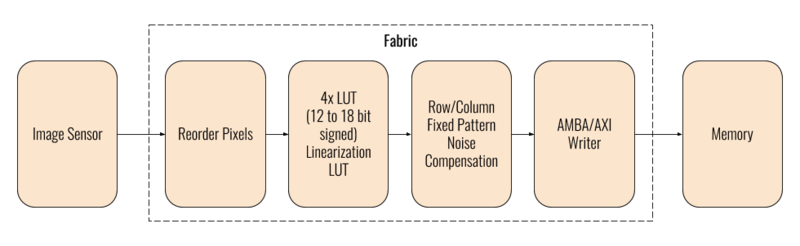
\includegraphics[height=5cm]{images/800px-AXIOM_Beta_Image_Acquisition_Pipeline}
\end{center}





\subsection{HDMI Image Processing/Output Pipeline}

\begin{center}
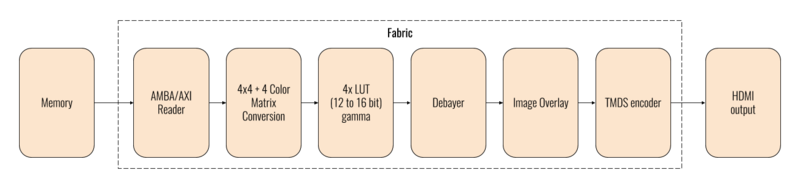
\includegraphics[height=4cm]{images/800px-AXIOM_Beta_HDMI_Image_Processing_Pipeline}
\end{center}





\subsection{SDI Image Processing/Output Pipeline}


ToDo - ETA Dec 2017.





\subsection{Image Processing Nodes}

\textbf{Debayering}\\

A planned feature is to generate this FPGA code block with "dynamic reconfiguration" meaning that the actual debayering algorithm can be replaced at any time by loading a new FPGA binary block at run-time. This tries to simplify creating custom debayering algorithms with a script like programming language that can be translated to FPGA code and loaded into the FPGA dynamically for testing. 

\textbf{Peaking}\\

Peaking marks high image frequency areas with colored dot overlays. These marked areas are typically the ones "in-focus" currently so this is a handy tool to see where the focus lies with screens that have lower resolution than the camera is capturing.\\

\textbf{Handy Custom Parameters:}\\

- color\\
- frequency threshold \\


\textbf{Potential Problems:}\\

There are sharper and softer lenses so the threshold depends on the glass currently used. For a sharp lens the peaking could show areas as "in-focus" if they actually aren't and for softer lenses the peaking might never show up at all because the threshold is never reached.\\
\section{Converting}

Overview text required.




\subsection{RAW12 to PGM}

Converts a video file recorded in AXIOM raw to a PGM image sequence and applies the darkframe (needs to be created beforehand).\\

Currently clips must go through ffmpeg before hdmi4k can read them:\\ 

\consoleCommand{ffmpeg -i CLIP.MOV -c:v copy OUTPUT.MOV}

To cut out a video between IN and OUT with ffmpeg but maintaing the original encoding data:

\consoleCommand{ffmpeg -i CLIP.MOV -ss IN\_SECONDS -t DURATION\_SECONDS -c:v copy OUTPUT.MOV}


\begin{lstlisting}[language=bash,morekeywords=$,keywordstyle=\bfseries,frame=none,xleftmargin=.25in,belowskip=2em, aboveskip=2em]
	hdmi4k
    HDMI RAW converter for Axiom BETA
     
    Usage:
      ./hdmi4k clip.mov
      raw2dng frame*.pgm [options]
     
    Calibration files:
      hdmi-darkframe-A.ppm, hdmi-darkframe-B.ppm:
      averaged dark frames from the HDMI recorder (even/odd frames)
     
    Options:
    -                   : Output PGM to stdout (can be piped to raw2dng)
    --3x3               : Use 3x3 filters to recover detail (default 5x5)
    --skip              : Toggle skipping one frame (try if A/B autodetection fails)
    --swap              : Swap A and B frames inside a frame pair (encoding bug?)
    --onlyA             : Use data from A frames only (for bad takes)
    --onlyB             : Use data from B frames only (for bad takes)
\end{lstlisting}





\subsection{RAW12 to DNG}

Converts AXIOM Beta raw image to DNG. 

   
\begin{lstlisting}[language=bash,morekeywords=$,keywordstyle=\bfseries,frame=none,xleftmargin=.25in,belowskip=2em, aboveskip=2em]
DNG converter for Apertus .raw12 files
 
Usage:
  ./raw2dng input.raw12 [input2.raw12] [options]
  cat input.raw12 | ./raw2dng output.dng [options]
 
Flat field correction:
 - for each gain (N=1,2,3,4), you may use the following reference images:
 - darkframe-xN.pgm will be subtracted (data is x8 + 1024)
 - dcnuframe-xN.pgm will be multiplied by exposure and subtracted (x8192 + 8192)
 - gainframe-xN.pgm will be multiplied (1.0 = 16384)
 - clipframe-xN.pgm will be subtracted from highlights (x8)
 - reference images are 16-bit PGM, in the current directory
 - they are optional, but gain/clip frames require a dark frame
 - black ref columns will also be subtracted if you use a dark frame.
 
Creating reference images:
 - dark frames: average as many as practical, for each gain setting,
   with exposures ranging from around 1ms to 50ms:
        raw2dng --calc-darkframe *-gainx1-*.raw12 
 - DCNU (dark current nonuniformity) frames: similar to dark frames,
   just take a lot more images to get a good fit (use 256 as a starting point):
        raw2dng --calc-dcnuframe *-gainx1-*.raw12 
   (note: the above will compute BOTH a dark frame and a dark current frame)
 - gain frames: average as many as practical, for each gain setting,
   with a normally exposed blank OOF wall as target, or without lens
   (currently used for pattern noise reduction only):
        raw2dng --calc-gainframe *-gainx1-*.raw12 
 - clip frames: average as many as practical, for each gain setting,
   with a REALLY overexposed blank out-of-focus wall as target:
        raw2dng --calc-clipframe *-gainx1-*.raw12 
 - Always compute these frames in the order listed here
   (dark/dcnu frames, then gain frames (optional), then clip frames (optional).
 
General options:
--black=%d          : Set black level (default: 128)
                      - negative values allowed
--white=%d          : Set white level (default: 4095)
                      - if too high, you may get pink highlights
                      - if too low, useful highlights may clip to white
--width=%d          : Set image width (default: 4096)
--height=%d         : Set image height
                      - default: autodetect from file size
                      - if input is stdin, default is 3072
--swap-lines        : Swap lines in the raw data
                      - workaround for an old Beta bug
--hdmi              : Assume the input is a memory dump
                      used for HDMI recording experiments
--pgm               : Expect 16-bit PGM input from stdin
 
--lut               : Use a 1D LUT (lut-xN.spi1d, N=gain, OCIO-like)
 
--totally-raw       : Copy the raw data without any manipulation
                      - metadata and pixel reordering are allowed.
 
Pattern noise correction:
--rnfilter=1        : FIR filter for row noise correction from black columns
--rnfilter=2        : FIR filter for row noise correction from black columns
                      and per-row median differences in green channels
--fixrn             : Fix row noise by image filtering (slow, guesswork)
--fixpn             : Fix row and column noise (SLOW, guesswork)
--fixrnt            : Temporal row noise fix (use with static backgrounds; recommended)
--fixpnt            : Temporal row/column noise fix (use with static backgrounds)
--no-blackcol-rn    : Disable row noise correction from black columns
                      (they are still used to correct static offsets)
--no-blackcol-ff    : Disable fixed frequency correction in black columns
 
Flat field correction:
--dchp              : Measure hot pixels to scale dark current frame
--no-darkframe      : Disable dark frame (if darkframe-xN.pgm is present)
--no-dcnuframe      : Disable dark current frame (if dcnuframe-xN.pgm is present)
--no-gainframe      : Disable gain frame (if gainframe-xN.pgm is present)
--no-clipframe      : Disable clip frame (if clipframe-xN.pgm is present)
--no-blackcol       : Disable black reference column subtraction
                      - enabled by default if a dark frame is used
                      - reduces row noise and black level variations
--calc-darkframe    : Average a dark frame from all input files
--calc-dcnuframe    : Fit a dark frame (constant offset) and a dark current frame
                      (exposure-dependent offset) from files with different exposures
                      (starting point: 256 frames with exposures from 1 to 50 ms)
--calc-gainframe    : Average a gain frame (aka flat field frame)
--calc-clipframe    : Average a clip (overexposed) frame
--check-darkframe   : Check image quality indicators on a dark frame
 
Debug options:
--dump-regs         : Dump sensor registers from metadata block (no output DNG)
--fixpn-dbg-denoised: Pattern noise: show denoised image
--fixpn-dbg-noise   : Pattern noise: show noise image (original - denoised)
--fixpn-dbg-mask    : Pattern noise: show masked areas (edges and highlights)
--fixpn-dbg-col     : Pattern noise: debug columns (default: rows)
--export-rownoise   : Export row noise data to octave (rownoise\_data.m)
--get-pixel:%d,%d   : Extract one pixel from all input files, at given coordinates,
                      and save it to pixel.csv, including metadata. Skips DNG output.
\end{lstlisting}
                       
                      
Example:                       

\consoleCommand{./raw2dng --fixrnt --pgm --black=120 frame%05d.dng}

\textbf{Compiling raw2dng}\\

Compiling raw2dng on a 64bit system requires the gcc-multilib package.\\

\textbf{Ubuntu:} 

    \consoleCommand{sudo apt-get install gcc-multilib}   
    
    
\textbf{openSUSE:}

    \consoleCommand{sudo zypper install gcc-32bit libgomp1-32bit}  
    
    
\textbf{AXIOM Beta:}

1. Acquire the source from \href{https://github.com/apertus-open-source-cinema/misc-tools-utilities/tree/master/raw2dng}{https://github.com/apertus-open-source-cinema/misc-tools-utilities/tree/master/raw2dng}.\\
2. Copy files to AXIOM Beta.\\
3. Remove \importantKeyword{-m32} from Makefile.\\
4. Run \importantKeyword{make} inside camera.\\                     
                      

\section{Maintenance}

Overview text required.





\subsection{Firmware}

The entire AXIOM Beta firmware is stored on a Micro SD card. This means that the camera's operating system can be swapped out easily and that external recovery of the camera entire software, in case anything went wrong eg. during flashing, is always possible.\\ 

It also means that experimental features can easily be tried and tested simply by popping in a different card into the camera. 





\subsubsection{Firmware Backup}

The entire camera firmware is stored on a Micro SD card plugged into the Microzed. To back-up the entire firmware we plug in the Micro SD card into a Linux PC and do the following:

1. Find out which device the micro SD card is: 

\consoleCommand{    cat /proc/partitions
    mount}

... should give you a list of all connected devices. Lets assume in our case that the card is /dev/sdc.\\


2. Make sure the card is unmounted (all 3 partitions): 

\consoleCommand{    umount /dev/sdc1
    umount /dev/sdc2
    umount /dev/sdc3t}
    
    
3. clone the entire card to a file: 

\consoleCommand{ddrescue /dev/sdc sdimage.img sdimage.log}

Here is a guide that covers doing the same on Mac and Windows: \href{http://raspberrypi.stackexchange.com/questions/311/how-do-i-backup-my-raspberry-pi}{http://raspberrypi.stackexchange.com/questions/311/how-do-i-backup-my-raspberry-pi}






\subsubsection{Firmware Restore}

Again you need to know the device path of your sd card, then (assuming in our case its /dev/sdb) run:

\consoleCommand{sudo dd if=sdimage.img of=/dev/sdb bs=4M}






\subsection{Image Sensor cleaning}

We are using the green sensor cleaning swabs:

\begin{center}

\includegraphics[height=5cm]{images/Green_Swabs_200X200_B}
\end{center}

It comes with two cleaning solutions: one for dust and one for any oil based residues (finger prints, etc.)\\

On this page we try to collect typical sensor contamination images, guides how to spot and get rid of them.\\

The best lighting conditions to spot contamination seems to be mid grey, you can take off or slightly turn the lens to make sure the contamination is not on any lens glass element.\\

Vertical streaks:\\

\begin{center}

\includegraphics[height=12cm]{images/Vertical-streaks}
\end{center}

These are the result of using the dust cleaning solution on the sensor. Likely the streaks are oil based contaminations. Use the red bottle "smear away" and a swap to clean the sensor. 

\section{Installations}

Overview text required.





\subsection{Installing a webserver}

\textbf{Installing required packages}\\

Make sure the AXIOM Beta is connected to the internet and then on the commandline:\\

Update mirrors database: 

\consoleCommand{pacman -Syy}

Install webserver: 

\consoleCommand{pacman -S lighttpd php php-cgi}

Start the webservice: 

\consoleCommand{systemctl start lighttpd}

Write any pending changes to the file system:

\consoleCommand{sync}





\subsection{Configuring a webserver}

This follows the guide from the lighttpd archlinux wiki page: \href{https://wiki.archlinux.org/index.php/lighttpd}{https://wiki.archlinux.org/index.php/lighttpd}

\consoleCommand{    mkdir /etc/lighttpd/conf.d/
    nano /etc/lighttpd/conf.d/cgi.conf}
    
... and place the following content in the file: 

\consoleCommand{
	server.modules += ( "mod\_cgi" )^^J
	^^J
	cgi.assign = (".pl"  => "/usr/bin/perl",^^J
					".cgi" => "/usr/bin/perl",^^J
                  ".rb"  => "/usr/bin/ruby",^^J
                  ".erb" => "/usr/bin/eruby",^^J
                  ".py"  => "/usr/bin/python",^^J
                  ".php" => "/usr/bin/php-cgi")^^J
	^^J     
	index-file.names += ("index.pl",   "default.pl",^^J
                         "index.rb",   "default.rb",^^J
                         "index.erb",  "default.erb",^^J
                         "index.py",   "default.py",^^J
                         "index.php",  "default.php")^^J
}  

For PHP scripts you will need to make sure the following is set in /etc/php/php.ini 

\consoleCommand{cgi.fix\_pathinfo = 1}

In your Lighttpd configuration file, /etc/lighttpd/lighttpd.conf add: 

\consoleCommand{include "conf.d/cgi.conf"}

Create a new configuration file /etc/lighttpd/conf.d/fastcgi.conf 

\consoleScript{
    # Make sure to install php and php-cgi. See:^^J                                                             
    # https://wiki.archlinux.org/index.php/Fastcgi\_and\_lighttpd#PHP^^J
     ^^J
    server.modules += ("mod\_fastcgi")^^J
     ^^J
    # FCGI server^^J
    # ===========^^J
    #^^J
    # Configure a FastCGI server which handles PHP requests.^^J
    #^^J
    index-file.names += ("index.php")^^J
    fastcgi.server = ( ^^J
        # Load-balance requests for this path...^^J
        ".php" => (^^J
            # ... among the following FastCGI servers. The string naming each^^J
            # server is just a label used in the logs to identify the server.^^J
            "localhost" => ( ^^J
                "bin-path" => "/usr/bin/php-cgi",^^J
                "socket" => "/tmp/php-fastcgi.sock",^^J
                # breaks SCRIPT\_FILENAME in a way that PHP can extract PATH\_INFO^^J
                # from it ^^J
                "broken-scriptfilename" => "enable",^^J
                # Launch (max-procs + (max-procs * PHP\_FCGI\_CHILDREN)) procs, where^^J
                # max-procs are "watchers" and the rest are "workers". See:^^J
                #^^J https://redmine.lighttpd.net/projects/1/wiki/frequentlyaskedquestions#How-many-php-CGI-processes-will-lighttpd-spawn ^^J
                "max-procs" => 4, # default value^^J
                "bin-environment" => (^^J
                    "PHP\_FCGI\_CHILDREN" => "1" # default value^^J
                )^^J
            )^^J
        )   ^^J
    )^^J
}

Make lighttpd use the new configuration file /etc/lighttpd/lighttpd.conf 

\consoleCommand{include "conf.d/fastcgi.conf"}

Restart lighttpd: 

\consoleCommand{systemctl restart lighttpd}

To test php create a file: /src/http/index.php with content:

\consoleCommand{    <?php
    phpinfo();
    ?>} 
    
... and open this IP address of your AXIOM Beta in a browser. If you see the php info status page everything worked successfully.     






\subsection{Installing AXIOM Beta Web GUI software}

Download this repository - \href{https://github.com/apertus-open-source-cinema/beta-software}{https://github.com/apertus-open-source-cinema/beta-software}\\

1. Copy all files from the http directory of the repository to your AXIOM Beta /srv/http/ directory.\\
2. Copy all files from the beta-scripts directory of the repository to your AXIOM Beta /root/ directory.\\ 

\textbf{Edit /etc/sudoers files:}\\

Under the line: 

\consoleCommand{root ALL=(ALL) ALL}

Add:

\consoleCommand{http ALL=(ALL) NOPASSWD: ALL}

This allows the http user to do anything with the system so it can be considered a security vulnerability - but for development this should not be an issue, later on we will define the http priviledges more securely.\\

For testing sudoers: 

\consoleCommand{sudo -u http sudo whoami}

If it returns \importantKeyword{root} then you are all set.\\

This should provide you with a working webbased GUI.\\

\textbf{Note :} \importantKeyword{lighttpd} does not start automatically when the AXIOM Beta boots, this still needs to be configured: 

\consoleCommand{systemctl enable lighttpd}

\textbf{Note also:} Opening any websites that read image sensor registers before initializing the image sensor \importantKeyword{kick\_manual.sh} will freeze/crash the camera. 







\subsection{Packet Manager Pacman}

Update all package definitions and the database from the Internet: 

\consoleCommand{pacman -Sy}

\textbf{Important:} Careful with upgrading existing packages. For example the Kernel used in the AXIOM Beta is custom developed - if you upgrade Arch Linux to the latest off the shelf Kernel you will BRICK your camera firmware.\\

\textbf{Install lighttp webserver on the Beta: }

\consoleCommand{pacman -S lighttpd}

Install PHP on the Beta: 

\consoleCommand{pacman -S php php-cgi}

Follow these instructions: \href{https://wiki.archlinux.org/index.php/lighttpd#PHP}{https://wiki.archlinux.org/index.php/lighttpd\#PHP}

Start the webserver: 

\consoleCommand{systemctl start lighttpd}

\section{Colour Science}

Overview text required.





\subsection{Black Calibration}

Black Calibration is a term that describes finding the sensor output value, per pixel, in the absence of any illumination.

It covers:\\

- Dark frame subtraction\\
- Dark current compensation\\
- Using black reference columns (called "optical black" by other manufacturers) to find the black level and fine-tune static offsets. \\

\textbf{Note:} Black reference columns can be used to reduce row noise as well. See Section 11.2 Pattern Noise.





\subsubsection{Calibration methods}





\paragraph{Dark Frame Subtraction}

This is a basic technique: take a picture with the lens cap on, and subtract it from your image. To make really sure no light is reaching the sensor, also cover the entire camera with something.\\ 

\textbf{How many dark frames?}\\

Problem: if you take only one dark frame, it will also contain read noise (assummed to be Gaussian and uncorrelated with the read noise from other frames). Therefore, subtracting only one image will actually increase the noise in the final output, by sqrt(2).\\

Solution: use a master dark frame, averaged from many images.\\

How many?\\

If you take N images, the signal will be multiplied by N, and the noise will be multiplied by sqrt(N). Therefore, the SNR will increase by log2(sqrt(N)) stops.\\

So, 16 dark frames will reduce the read noise in the dark frame by 2 stops, 64 frames by 3 stops, and 256 frames by 4 stops.\\

Okay, but how much noise will be added to the output image?\\

Let's say the read noise stdev in one image is r, so a dark frame averaged from N frames will have noise \consoleCommand{stdev = r/sqrt(N)}. Therefore, the noise in the output image will be: \consoleCommand{sqrt(r\^2 + r\^2/N) = r * sqrt(1 + 1/N)}.\\

Check it in octave:\\ 

\begin{lstlisting}[language=bash,morekeywords=$,keywordstyle=\bfseries,frame=none,xleftmargin=.25in,belowskip=2em, aboveskip=2em]
    octave:1>  N = 4;
    octave:2>  a = randn(1,1000000);    # one Gaussian noise sample, with mean=0 and stdev=1
    octave:3>  b = randn(N,1000000);    # N noise samples
    octave:4>  std(a + mean(b))         # add one noise sample to N averaged noise samples
    ans =  1.1174
    octave:5>  sqrt(1 + 1/4)            # compare with the theoretical result
    ans =  1.1180
\end{lstlisting}

So, it seems that averaging a small number of dark frames will not introduce significant noise in your images (4 should be enough if you are in a hurry, and 16 should give a very good result).\\

Example: one dark frame at 6ms x1 (same image as above), vs 4 darkframes at 6ms, averaged.\\

\begin{center}

\includegraphics[height=5cm]{images/blackframes-gainx1-offset2047-5ms-01}
\end{center}

\begin{center}

\includegraphics[height=5cm]{images/darkavg-5ms}
\end{center}

What about camera settings?\\

Unfortunately, dark frames depend on many camera settings: analog gain (ISO), exposure, other sensor settings like offset, black sun protection, PLR configuration and so on. Temperature is a variable as well.\\

Luckily, the dependence on exposure appears to be linear, so we can take calibration frames at various exposures, combine them into a single dark frame, adjust it for the dark current and use it for the entire range of exposure settings (hopefully). We'll discuss that in the next section.\\ 

\textbf{Dark current}\\

Let's look at some dark frames: gain x1, exposures 1.2ms, 6ms and 78ms. Notice they get brighter as exposure increase.\\

\begin{center}

\includegraphics[height=5cm]{images/blackframes-gainx1-offset2047-1ms-01}
\end{center}

\begin{center}

\includegraphics[height=5cm]{images/darkavg-5ms}
\end{center} 

\begin{center}

\includegraphics[height=5cm]{images/blackframes-gainx1-offset2047-64ms-01}
\end{center}

The overall brightness in the dark frame changes with exposure in a linear fashion. We'll try to account for this in two ways: with a simple scalar value, and with a per-pixel correction.\\

The values in the black reference columns do not appear to compensate for the dark current, so we'll need to do it ourselves.\\

By identifying the dark current, we will be able to compute a dark frame that is applicable to any usual exposure time, but we are going to store only one or two reference frames for each gain. First reference frame will be called a bias frame (a zero-length exposure, that would contain only static black offsets), and the second reference frame, if used, will be called a dark current frame.\\

Dark current cannot be fully corrected because, while its stationary value can be measured and subtracted, it also introduces photon noise. Roger Clark explains it better:\\ 

\textit{"Dark current is temperature dependent and most modern CMOS digital cameras, circa 2008 and later have on sensor dark current subtraction, but while the dark current level is subtracted, the noise from the dark current still accumulates."} - Source: \href{http://www.clarkvision.com/reviews/how-to-interpret-reviews/}{http://www.clarkvision.com/reviews/how-to-interpret-reviews/}

\textbf{Simple correction}\\

Experimentally, we have found the dark frame changes with exposure at roughly 0.065 digital units for each ms. This value is multiplied by analog gain. To find this value, take the dark frames at different exposure times (say 1...50 ms), then do a linear fit for the frame average (or median).\\

Command-line:

\consoleCommand{raw2dng *x1*.raw12 --calc-darkframe}

Example: a dark frame created from 256 exposures, between 1.2ms and 77ms, without using black reference columns. The image was adjusted (with a constant offset) to match a zero-length exposure, so calling it bias frame may be a good idea. If we use it to correct the individual dark frames, we should no longer see a variation in overall brightness. 

\consoleCommand{    Averaged 256 frames exposed from 1.19 to 76.79 ms.
    Dark current: 0.0653 DN/ms}
    
Image sequence: bias frame, single dark frames at exposures 1.2, 6 and 77 ms, corrected with the bias frame and the (scalar) dark current average. All files scaled to show a range of 60 DN, but the master dark frame has a different offset than the others.     


\begin{center}

\includegraphics[height=5cm]{images/darkframe-x1-no-blackcol-256}
\end{center}

\begin{center}

\includegraphics[height=5cm]{images/blackframes-gainx1-offset2047-1ms-01-simple-darkframe-no-blackcol}
\end{center} 

\begin{center}

\includegraphics[height=5cm]{images/blackframes-gainx1-offset2047-5ms-01-simple-darkframe-no-blackcol}
\end{center}

\begin{center}

\includegraphics[height=5cm]{images/blackframes-gainx1-offset2047-64ms-01-simple-darkframe-no-blackcol}
\end{center}





\paragraph{Dark Current Non-uniformity Correction}

One common use of bias frames is for scaling dark frames. By subtracting a bias frame from a dark frame, you end up with a thermal frame. A thermal frame contains pixel values showing just the effect of dark current. Because dark current in any given pixel accumulates at a constant rate, a thermal frame allows you to predict with reasonable accuracy how much dark current there would be for different length exposures. However, given the opportunity, you’re always better off taking dark frames that match the exposure times of your light frames.\\

\href{http://qsimaging.com/ccd_noise_measure.html}{http://qsimaging.com/ccd\_noise\_measure.html}{Source}: \\

\textit{"Dark current non-uniformity is a noise that results from the fact that each pixel generates a slightly different amount of dark current. This noise can be eliminated by subtracting a dark reference frame from each image. The dark reference frame should be taken at the same temperature and with the same integration time as the image."} - Source: \href{https://www.photometrics.com/resources/learningzone/darkcurrent.php}{https://www.photometrics.com/resources/learningzone/darkcurrent.php}\\

\textit{"Dark noise is not random; in fact, it is highly repeatable. A given photosite on a sensor will accumulate almost exactly the same amount of dark noise from one exposure to the next, as long as temperature and exposure duration do not vary."}\\

So, rather than using a single scalar value (0.06 dn/ms/gain) for all pixels, we can try finding the individual dark current for each pixel. Instead of doing a linear fit on the overall dark frame brightness (vs exposure), we will do the linear fit per pixel. We'll have to acquire a lot more dark frames to compute a good result, but it might be worth the trouble.\\

Command-line:\\

\consoleCommand{raw2dng *x1*.raw12 --calc-dcnuframe}

Example: bias frame (static offset) and dark current frame (exposure-dependent offset). Notice the bias frame looks quite similar to the previous one, but a little darker. The median value of the dark current frame is, unsurprisingly, 0.0645 DN/ms. 

\begin{center}

\includegraphics[height=5cm]{images/darkframe-x1-no-blackcol-darkcurrent-256}
\end{center}

\begin{center}

\includegraphics[height=5cm]{images/dcnuframe-x1-no-blackcol-darkcurrent-256}
\end{center}

Individual dark frames (1.2, 6 and 77 ms) adjusted with dark current nonuniformity: 

\begin{center}

\includegraphics[height=5cm]{images/blackframes-gainx1-offset2047-1ms-01-darkcurrent-no-blackcol}
\end{center}

\begin{center}

\includegraphics[height=5cm]{images/blackframes-gainx1-offset2047-5ms-01-darkcurrent-no-blackcol}
\end{center}

\begin{center}

\includegraphics[height=5cm]{images/blackframes-gainx1-offset2047-64ms-01-darkcurrent-no-blackcol}
\end{center}

No obvious improvement in the test images, so why bother?\\

Let's correct all these 256 dark frames and check a few indicators: median, stdev, row noise and column noise.\\ 

Dark frame + scalar dark current: 
\begin{center}
%\includegraphics[height=5cm]{images/darkframe-check-x1-256-simple}
\end{center}


Dark frame + dark current frame:
\begin{center}
%\includegraphics[height=5cm]{images/darkframe-check-x1-256-dcnu}
\end{center}

You may notice:\\

- Median (black level) variation: noticeable improvement with the second method.\\
- stdev (overall noise): minor improvement at extreme settings.\\
- Row noise: identical with both methods.\\
- Column noise: small improvement with the second method.\\

Indeed, the more complex method appears just a tiny bit better than the simpler one.\\





\paragraph{Dark Current Measurement From Hot Pixels}

A very interesting idea can be found here - \href{https://www.photonics.com/Article.aspx?AID=44298}{https://www.photonics.com/Article.aspx?AID=44298} ... where hot pixels can be used to measure the amount of dark current and scale it properly. This will probably account for changes in temperature, and may work at very long exposures without actually having to calibrate the camera in these conditions. Genius, if you ask me. 





\paragraph{Black Reference Columns}

This sensor has 8+8 columns that can be used for calibrating the black levels; they are also useful for reducing the dynamic row noise.\\

Experimentally, we have noticed that odd rows have slightly different statistics (noise level, offset, gain), compared to even rows. This happens in both the black columns and the active area, and it may indicate two parallel circuits used for readout, each having slightly different electrical response.\\

Therefore, it may be wise to process the black columns for odd and even rows separately, which should already fix some issues like static row noise, or the need for green equilibration.\\

In raw2dng, this correction is enabled by default, as long as you use a dark frame. You can turn it off with \importantKeyword{--no-blackcol}, if you want. \\





\paragraph{Black Level}

The sensor has two registers that can be used to adjust the black level: one for odd rows, another for even rows. This confirms our finding about two parallel readout circuits.\\

You might be tempted to adjust the black level to 0 (like Nikon does). Please don't. Here's why:\\

- If you adjust the offset until the black level becomes roughly 0, you will clip all the data below this level. Good luck subtracting a dark frame after that.\\
- Even if you change the level after doing all the black corrections, you may still have useful data below zero. You will need it when stacking multiple frames, or when doing noise reduction.\\

Just FYI, there is a hack for Nikon cameras that moves the black level above 0. See \href{https://landingfield.wordpress.com/2014/05/13/teaser-nikon-dslr-black-point-hack-for-astrophotography/}{https://landingfield.wordpress.com/2014/05/13/teaser-nikon-dslr-black-point-hack-for-astrophotography/} \\

... Sample photos can be found \href{https://www.cloudynights.com/topic/473696-rho-ophiuchi-with-nikon-hacked-black-level/}{here} or \href{https://nikonhacker.com/viewtopic.php?t=2548&p=18449#p17973}{here}.

We recommend setting the offset so that only a few isolated pixels (if any) reach the value of 0. A black offset of 2047 (registers 87/88) is a good choice. You won't lose any dynamic range by doing that.\\

On most recent Canon DSLRs, black level is 2048. That's a little on the large side, but it's a good thing. Some may argue that you may lose 2 stops or more of dynamic range by doing that (reading - \href{https://www.reddit.com/r/photography/comments/3q4tnz/how_to_correctly_push_5_stops_with_canon/cwcbyb5/}{https://www.reddit.com/r/photography/comments/3q4tnz/how\_to\_correctl\_push\_5\_stops\_with\_canon/cwcbyb5/} ), but this is wrong. On Canons, the raw output is 14-bit, so by setting the offset to 2048 instead of 0, the useful range will be "just" log2(16384-2048) = 13.8 bits, instead of 14. So, yeah, you lose 0.2 bits from the ADC range.\\

With the black offset of 2047 on the CMV12K, the black level ends up at around 150, so you lose a whooping 0.05 bits from the 12-bit range.\\

\textbf{Note:} for easier processing, raw2dng shifts the raw data in order to fix the black level at 128.\\

\textbf{Note also:} Row noise correction from black columns detailed in 11.2 Pattern Noise.
 




\subsubsection{Checking Black Level}

You may wonder: after all these corrections, did we get the right black level? Can we render shadow detail correctly?\\

A possible criteria for checking: if we have two images of the same scene, taken with different exposures, we should be able to match those in postprocessing by simply dragging the exposure slider. For example, if we have one image at 5ms and another one at 20ms, we would set the exposure to +2 EV on the first image - the results should be pretty much identical, except for noise (and clipped highlights, if we weren't careful with the exposure). \\

Of course, that will work once we know the sensor Response Curves (See 11.5).\\

To check how well the images can be exposure-compensated, we could evaluate (and minimize) one of those error metrics: 

\begin{lstlisting}[language=bash,morekeywords=$,keywordstyle=\bfseries,frame=none,xleftmargin=.25in,belowskip=2em, aboveskip=2em]
    a  = dark\_image - black\_level;
    b  = bright\_image - black\_level;
    e1 = norm(a*expo\_ratio - b);
    e2 = abs(median((b ./ a)(:)) - expo\_ratio)
    e3 = mad(log2((b ./ a)(:)));
\end{lstlisting}

First metric checks the difference between the two images, where the darkest one was adjusted by scaling (gain) to match the brightest one. Second metric computes the ratio between the two images at each pixel, and checks its median value vs the expected value. Third one checks the variation of per-pixel ratios between the two images, in stops, ignoring the expected value - this metric could be useful if we suspect the exposure controls may not be accurate.\\

\begin{center}
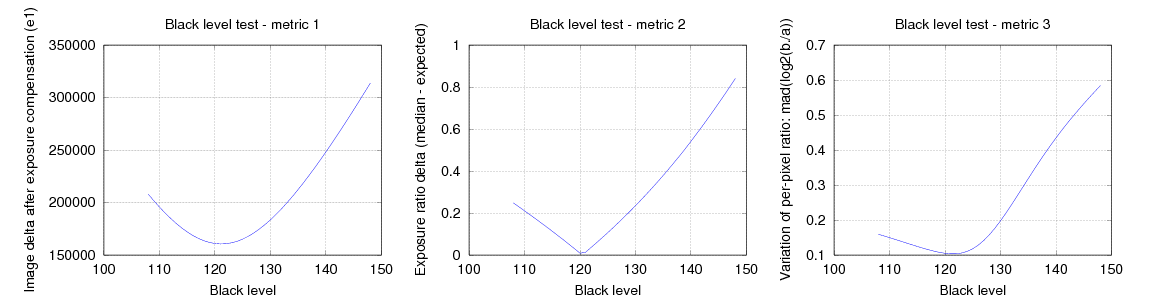
\includegraphics[height=5cm]{images/black_check}
\end{center}

With all 3 methods, minimization indicates a black level of around 120-122 (expected 128), so there's still something missing with our calibration. This is confirmed by missing details in very dark areas (crushed blacks) on some sample images.\\ 

On the same test image, the response curve estimated from the grayscale IT8 reference data indicates a black level of 129. 

On the same test image, the response curve estimated with the Robertson02 algorithm indicates a black level of 124 (See 11.5).\\

Who is right?\\

The sensor also has a strange behavior - something we have called the "Black Hole" anomaly: in very dark areas, sensor output decreases with exposure time. This might give a clue for solving this mystery.\\

\begin{center}

\includegraphics[height=5cm]{images/blackhole}
\end{center}





\subsubsection{Calibration Pipeline}

- Use black reference columns to find the black levels for odd and even rows.\\
- Subtract dark offset and dark current.\\
- Use variations in black reference columns to reduce row noise.\\ 

These operations should be simple enough to be implemented in FPGA, as real-time corrections. 





\subsubsection{Calibration Procedure}

\textbf{Quick calibration}\\

Acquire 16 dark frames, gain x1, exposures between 1 and 50 ms, save them under the 'darkframes' subdirectory, then run: 

\consoleCommand{raw2dng darkframes/*x1*.raw12 --calc-darkframe --swap-lines}

Result: darkframe-x1.pgm.\\

Repeat for other gains if needed.\\ 


\textbf{Accurate calibration, with dark current nonuniformity}

Acquire 256 dark frames, gain x1, exposures between 1 and 64 ms in linear increments (4 images at each setting), save them under the 'darkframes' subdirectory, then run: 

\consoleCommand{raw2dng darkframes/*x1*.raw12 --calc-dcnuframe --swap-lines}

Result: darkframe-x1.pgm and dcnuframe-x1.pgm.\\

Repeat for other gains if needed. \\

\textbf{Checking the calibration}\\

You can verify the calibration by rendering the same individual dark frames, this time corrected, to check the residuals. Or, even better, acquire a new set of dark frames at the same settings, and check those instead: 

\consoleCommand{raw2dng darkframes/*x1*.raw12 --check-darkframe --swap-lines}

You will see the average value, pixel noise and row/column noise levels (both absolute and relative to pixel noise) for each dark frame. Example:

\consoleCommand{    Average     : 127.48
    Pixel noise : 2.48
    Row noise   : 0.61 (24.6\%)
    Col noise   : 0.05 (2.2\%)}
    
Using the reference frames to correct raw12 files.\\

1. Place the calibration files in the working directory.\\
2. Make sure your \importantKeyword{.raw12} images contain a metadata block.\\
3. raw2dng will recognize the dark frames and use them for correcting your image. \\
   
\consoleCommand{    cp /path/to/darkframes/*-x[1-4].pgm .
    raw2dng *.raw12 --swap-lines}
    
\textbf{Note:} you need --swap-lines as an workaround for an old bug introduced in the Beta, but wasn't fixed yet in the FPGA.\\    
    
This is not exactly useful when dealing with multiple folders, so until we'll have a better way to organize the calibration frames, you may try an alternative workflow:\\

1. Place the calibration files in some directory (let's call it "calibration directory")\\.
2. Make sure your .raw12 images contain a metadata block.\\
3. Use paths when passing input files raw2dng (the output files will be saved in the same directory as the input file).\\

\consoleCommand{    cd /path/to/darkframes
    ls *.pgm
      darkframe-x1.pgm       dcnuframe-x1.pgm       ...
    raw2dng /path/to/images/*.raw12 --swap-lines}
     
    
\textbf{Example}

Showing half-res image crops pushed by 4 stops (ufraw-batch --wb=auto --exposure=4 --shrink=2).

- Top left: raw sensor data (adjusted black level manually).\\
- Top right: corrected with dark frame, scalar dark current, no black columns.\\
- Bottom left: corrected with dark frame, dark current frame, no black columns.\\
- Bottom right: corrected with dark frame, dark current frame, black columns enabled.\\

\textbf{Note:} in the raw data, even and odd rows have different black offsets; that's why we have wrong colors. \\

\begin{center}
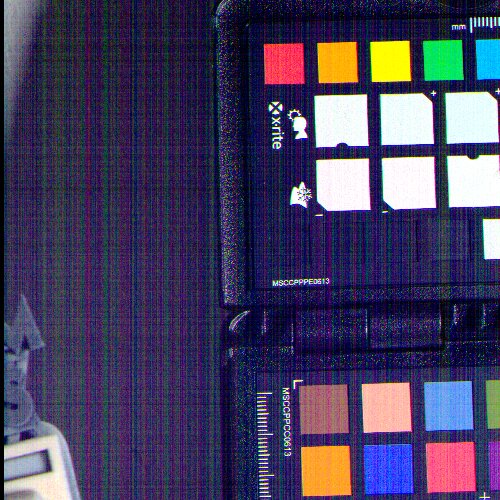
\includegraphics[height=5cm]{images/10ms+4-totally-raw-crop}
\end{center}

\begin{center}
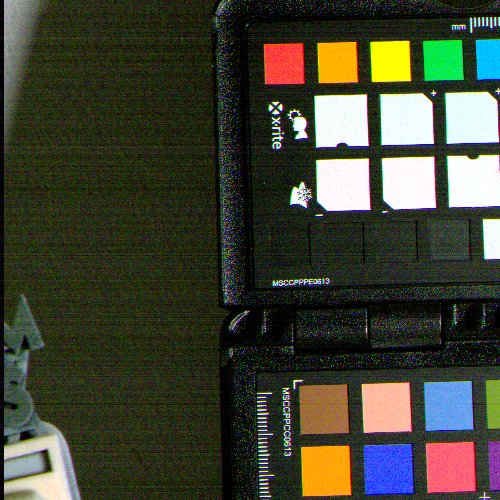
\includegraphics[height=5cm]{images/10ms+4-no-blackcol-crop}
\end{center}

\begin{center}
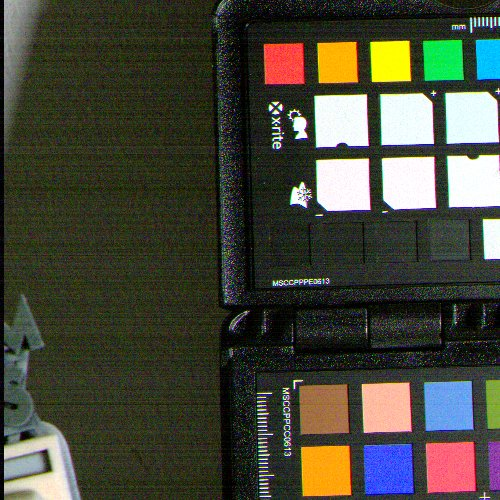
\includegraphics[height=5cm]{images/10ms+4-darkcurrent-no-blackcol-crop}
\end{center}

\begin{center}
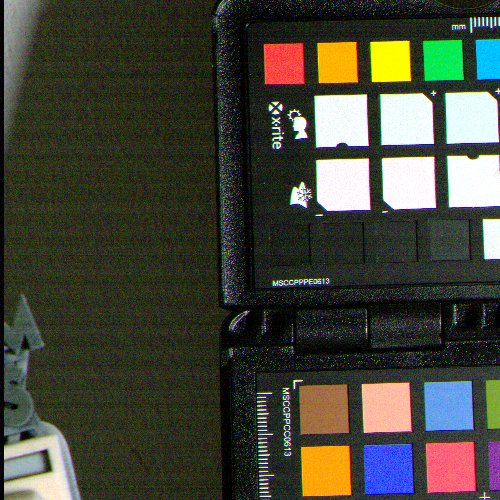
\includegraphics[height=5cm]{images/10ms+4-darkcurrent-crop}
\end{center}


    

\subsection{Pattern Noise}

General info about pattern noise can be found here - \href{http://theory.uchicago.edu/~ejm/pix/20d/tests/noise/#patternnoise}{http://theory.uchicago.edu/~ejm/pix/20d/tests/noise/\#patternnoise} \\

The CMV12000 sensor suffers from dynamic row noise.\\

That means, a scalar offset gets added to each row. The offset is not correlated between different frames, so we can't remove it using a calibration frame (dark frame or whatever).\\

One can observe this noise by looking at the difference between two images taken at identical settings. There are two main components that appear obvious in such a difference frame: random noise (per pixel, increases on brighter pixels) and row noise (per line). \\

\begin{center}
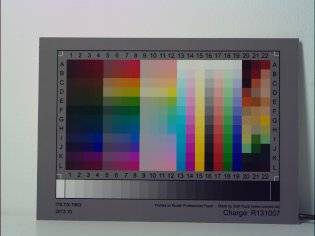
\includegraphics[height=5cm]{images/it8-gainx1-offset2047-20ms-01}
\end{center}

\begin{center}

\includegraphics[height=5cm]{images/it8-gainx1-offset2047-20ms-01-minus-02-small}
\end{center}




\subsubsection{Correction Methods}

There are two ways to deal with this noise, after performing Black Calibration (See 11.1)\\

- Use info from black reference columns to reduce dynamic row noise without guessing anything (fast, can be implemented in real-time, see Raw Preprocessing).\\
- Use denoising techniques to reduce the remaining row noise (the guesswork part, slow).\\

\textbf{Reducing row noise using black reference columns}

See \href{http://github.com/apertus-open-source-cinema/misc-tools-utilities/commit/48de47b2a544dc32bbd5a8fd7701bb44a31ea850#diff-624053a553f49c0036b4d31282e58b2fR301}{http://github.com/apertus-open-source-cinema/misc-tools-utilities/commit/48de47b2a544dc32bbd5a8fd7701bb44a31ea850\#diff-624053a553f49c0036b4d31282e58b2fR301}

The application note AN01 from CMOSIS says:\\

\textit{"The noise is also present in the black reference columns (8 left and 8 right), so when enabled (reg 89[15] = 1), these can be used for row noise correction by for example making a relative row profile of these black columns and subtract this from the image."}\\

However, simply subtracting each row average of the black columns from our image is not going to work. Here's why:\\

Kalman filter theory: \href{http://robocup.mi.fu-berlin.de/buch/kalman.pdf}{http://robocup.mi.fu-berlin.de/buch/kalman.pdf} \\

From page 3, if we know how noisy our estimations are, the optimal weights are inversely proportional with the noise variances:\\

\consoleCommand{x\_optimal = (x1 * var(x2) + x2 * var(x1)) / (var(x1) + var(x2))} 

Here, let's say R = x1 is row noise (stdev = 1.6 at gain=x1) and x2 is black column noise. 

\begin{lstlisting}[language=bash,morekeywords=$,keywordstyle=\bfseries,frame=none,xleftmargin=.25in,belowskip=2em, aboveskip=2em]
    R = x1
    B = mean(black\_col') = R + x2 =>  x2 = B - R
    x2 can be estimated as mean(black\_col') - mean(active\_area')
    stdev(x2) = 1.3.
\end{lstlisting}

We want to find k that minimizes var(R - k*B). 

\begin{lstlisting}[language=bash,morekeywords=$,keywordstyle=\bfseries,frame=none,xleftmargin=.25in,belowskip=2em, aboveskip=2em]
    var(R - k*B) = var(x1 * (1-k) - x2 * k),
    => k = var(x1)) / (var(x1) + var(x2).
\end{lstlisting}

In particular, for gain = x1, k = 1.6\^2 / (1.6\^2 + 1.3\^2) = 0.6.\\

So, we don't have to simply subtract the black columns. Rather, we'll subtract the static offset (median value) first, and then, we'll subtract the remaining variations multiplied by 0.6 at gain=x1.\\

Things get a little more complex because the static offset is different on odd and even rows, and it also appears to change from the left side to right side of the frame. More details on the \textbf{Raw Preprocessing} page.\\

\textbf{Fixed frequency perturbation in black columns }\\

A closer look at the frequency spectrum of the black columns, compared to the spectrum of the row noise from a dark frame, revealed a strong fixed-frequency component present only in the black columns. Attempting to fix row noise with the above procedure would introduce some of this fixed frequency component in the main image as well.\\

In the example image from below, this component has a frequency of 1/41.27 pixels-1, with an amplitude of 1.14 DN. The value is different in other test images, and appears to be consistent in the images taken during the same experiment. It doesn't change with exposure time. Cause is unknown. \\

TODO: detailed analysis, FFT graphs...\\

We'll attempt to filter out this perturbation from the black columns before using them for reducing row noise.\\

Good news: after removing this perturbation, the optimal black columns multiplier increases to about 0.8 :) \\

\textbf{Using nearby rows to reduce the row noise even more}\\

Maybe some nearby rows could offer some hints about the row offset on the line being analyzed?\\

Looks like yes. Trying to write the row noise as a linear combination of row averages from black columns, using linear regression, not just the ones from the same row, but also from nearby rows, and discarding very small coefficients, gives the following filter:\\

 \begin{lstlisting}[language=bash,morekeywords=$,keywordstyle=\bfseries,frame=none,xleftmargin=.25in,belowskip=2em, aboveskip=2em]
    (y % 2)
       ?
         black\_col[y-1] *  0.24 +
         black\_col[y]   *  0.63
       :
         black\_col[y]   *  0.38 +
         black\_col[y+1] *  0.43
\end{lstlisting}

What's interesting: on even rows, row noise (in the active area) depends on the black column average from the same row, but also on the black column average from the previous row. But on odd rows, it depends on the black column average from the same row and the next row. This probably means they are processed in pairs, and there is some common perturbation that affects both of them.\\

This gives a minor improvement (0.6 -> 0.5). \\

\textbf{Exploiting differences in green channels}

The two green channels are expected to be nearly identical, except for high-frequency details like sharp edges. That means, if we take the median difference on each row, we expect to get zero. In practice, we get some nonzero values. We could try to see if there is any correlation between those green channel differences and our row noise.\\

Let's extract only the green channels from an image: the result will be W x H/2. Let's define green\_delta(lag) = row\_median(green - circshift(green,-lag)). That means, from each green row, subtract some nearby green row, and take the median difference. We'll compute this at lags -2, -1, 1, 2, mapped to array indices 0, 1, 2, 3.\\

Linear regression gives an ugly FIR filter that looks like this: \\

\begin{lstlisting}[language=bash,morekeywords=$,keywordstyle=\bfseries,frame=none,xleftmargin=.25in,belowskip=2em, aboveskip=2em]
    (y % 2)
       ?
         black\_col[y-2]    * 0.17 +
         black\_col[y-1]    * 0.14 +
         black\_col[y+0]    * 0.17 +
         black\_col[y+1]    * 0.16 +
         black\_col[y+2]    * 0.14 +
         green\_delta[0][y] * 0.22 +
         green\_delta[1][y] * 0.31 +
         green\_delta[2][y] * 0.38
       :
         black\_col[y-2]    * 0.12 +
         black\_col[y-1]    * 0.13 +
         black\_col[y+0]    * 0.14 +
         black\_col[y+1]    * 0.14 +
         black\_col[y+2]    * 0.12 +
         black\_col[y+3]    * 0.12 +
         green\_delta[0][y] * 0.33 +
         green\_delta[3][y] * 0.32
\end{lstlisting}

As weird as it looks, it seems to work!\\

Improvement (over the "Kalman" scaling of black columns): 0.6 -> 0.3.\\ 



\textbf{Reducing the remaining row noise by image filtering}\\

Basic algorithm:\\

1. Filter the image with an edge-aware vertical blur (bilateral filter on pixels from the same column)\\
2. Subtract the blurred image; the residuals will reveal the row noise (see example)\\
3. Mask out highlights and strong edges\\
4. Take the median value from each row of the residuals image\\
5. Subtract these values from each row of the original image \\

Source: \href{https://github.com/apertus-open-source-cinema/misc-tools-utilities/blob/master/raw2dng/patternnoise.c}{https://github.com/apertus-open-source-cinema/misc-tools-utilities/blob/master/raw2dng/patternnoise.c} \\





\subsubsection{Usage}

The methods discussed here are implemented here = \href{https://github.com/apertus-open-source-cinema/misc-tools-utilities/tree/master/raw2dng}{https://github.com/apertus-open-source-cinema/misc-tools-utilities/tree/master/raw2dng} \\

- Black reference columns are used by default, as long as you use a dark frame (since this method is fast and has no side effects)\\
- To reduce the remaining row noise, use \importantKeyword{raw2dng --fixrn}\\
- If the image also suffers from column noise, use \importantKeyword{raw2dng --fixpn} \\

Troubleshooting or checking the effectiveness of each step:

- Disable row noise reduction from black columns, but use the static offsets: \importantKeyword{--no-blackcol-rn}\\
- Disable fixed frequency correction for black columns: \importantKeyword{--no-blackcol-ff}\\
- Disable black reference columns completely: \importantKeyword{--no-blackcol} (you need to compute new darkframes if you use this)\\ 

Tip: the algorithm for filtering row noise is also available in MLVFS, so you can use it on MLV videos (recorded with Magic Lantern) as well. See - \href{http://www.magiclantern.fm/forum/index.php?topic=13152}{http://www.magiclantern.fm/forum/index.php?topic=13152}





\subsubsection{Tests on a dark frame}

Checking a single 10ms dark frame, corrected using 256 exposures between 1.2ms and 77ms, various settings. Showing only noise measurements.

\begin{lstlisting}[language=bash,morekeywords=$,keywordstyle=\bfseries,frame=none,xleftmargin=.25in,belowskip=2em, aboveskip=2em]
    # raw data without any processing
    raw2dng blackframes-gainx1-offset2047-10ms-01.raw12 --swap-lines --no-darkframe --check-darkframe
      Average     : 190.35
      Pixel noise : 7.14
      Row noise   : 5.29 (74.1%)
      Col noise   : 5.41 (75.7%)
\end{lstlisting}

\begin{lstlisting}[language=bash,morekeywords=$,keywordstyle=\bfseries,frame=none,xleftmargin=.25in,belowskip=2em, aboveskip=2em]
    # disable black columns, simple darkframe
    raw2dng *x1*.raw12 --calc-darkframe --no-blackcol --swap-lines
    raw2dng blackframes-gainx1-offset2047-10ms-01.raw12 --swap-lines --no-blackcol --check-darkframe
      Average     : 140.33
      Pixel noise : 3.08
      Row noise   : 1.33 (43.0%)
      Col noise   : 0.09 (3.0%)
\end{lstlisting}

\begin{lstlisting}[language=bash,morekeywords=$,keywordstyle=\bfseries,frame=none,xleftmargin=.25in,belowskip=2em, aboveskip=2em]
    # disable black columns, enable dark current frame
    raw2dng *x1*.raw12 --calc-dcnuframe --no-blackcol --swap-lines
    raw2dng blackframes-gainx1-offset2047-10ms-01.raw12 --swap-lines --no-blackcol --check-darkframe
      Average     : 142.46
      Pixel noise : 3.06
      Row noise   : 1.32 (43.1%)
      Col noise   : 0.08 (2.5%)
\end{lstlisting}

\begin{lstlisting}[language=bash,morekeywords=$,keywordstyle=\bfseries,frame=none,xleftmargin=.25in,belowskip=2em, aboveskip=2em]
    # dark current frame, use only static offsets from black columns
    raw2dng *x1*.raw12 --calc-dcnuframe --swap-lines
    raw2dng blackframes-gainx1-offset2047-10ms-01.raw12 --swap-lines --no-blackcol-rn --check-darkframe
      Average     : 127.46
      Pixel noise : 3.06
      Row noise   : 1.39 (45.4%)
      Col noise   : 0.10 (3.2%)
\end{lstlisting}

\begin{lstlisting}[language=bash,morekeywords=$,keywordstyle=\bfseries,frame=none,xleftmargin=.25in,belowskip=2em, aboveskip=2em]
    # dark current frame, enable black columns, don't remove the fixed frequency component from black columns
    raw2dng blackframes-gainx1-offset2047-10ms-01.raw12 --swap-lines --no-blackcol-ff --check-darkframe
      Average     : 127.46
      Pixel noise : 2.90
      Row noise   : 0.82 (28.2%)
      Col noise   : 0.10 (3.3%)
\end{lstlisting}

\begin{lstlisting}[language=bash,morekeywords=$,keywordstyle=\bfseries,frame=none,xleftmargin=.25in,belowskip=2em, aboveskip=2em]
    # dark current frame, enable black columns, remove the fixed frequency component (default setting)
    raw2dng blackframes-gainx1-offset2047-10ms-01.raw12 --swap-lines --check-darkframe
      Average     : 127.46
      Pixel noise : 2.85
      Row noise   : 0.61 (21.4%)
      Col noise   : 0.10 (3.4%)
\end{lstlisting}

\begin{lstlisting}[language=bash,morekeywords=$,keywordstyle=\bfseries,frame=none,xleftmargin=.25in,belowskip=2em, aboveskip=2em]
    # also enable --fixrn (aggressive correction)
    raw2dng blackframes-gainx1-offset2047-10ms-01.raw12 --swap-lines --fixrn --check-darkframe
      Average     : 127.42
      Pixel noise : 2.79
      Row noise   : 0.12 (4.1%)
      Col noise   : 0.10 (3.5%)
\end{lstlisting}

So, row noise was reduced from 1.33 (after dark frame correction) to 0.61 after using the black reference columns.\\

If it's still noticeable, \importantKeyword{--fixrn} should bring it to very low levels, unless you have strong horizontal lines in the image, which might trick the algorithm.\\

Some experimental row noise filters:\\

\begin{lstlisting}[language=bash,morekeywords=$,keywordstyle=\bfseries,frame=none,xleftmargin=.25in,belowskip=2em, aboveskip=2em]
    % 2-tap FIR, separate for odd/even rows
    raw2dng blackframes-gainx1-offset2047-10ms-01.raw12 --swap-lines --rnfilter=1 --check-darkframe
      Average     : 127.44
      Pixel noise : 2.84
      Row noise   : 0.51 (18.1%)
      Col noise   : 0.10 (3.4%)
\end{lstlisting}

\begin{lstlisting}[language=bash,morekeywords=$,keywordstyle=\bfseries,frame=none,xleftmargin=.25in,belowskip=2em, aboveskip=2em]
    % that ugly FIR that also looks at green channel differences
    raw2dng blackframes-gainx1-offset2047-10ms-01.raw12 --swap-lines --rnfilter=2 --check-darkframe
      Average     : 127.47
      Pixel noise : 2.81
      Row noise   : 0.31 (11.1%)
      Col noise   : 0.10 (3.4%)
\end{lstlisting}


\textbf{Example}

Showing half-res image crops pushed by 4 stops (ufraw-batch --wb=auto --exposure=4 --shrink=2).\\


- Left: raw sensor data (adjusted black level manually).\\
- Right: after dark frame and dark current subtraction, but without correction from black columns.\\
- Note: in the raw data, even and odd rows have different black offsets; that's why we have wrong colors.\\ 

\begin{center}
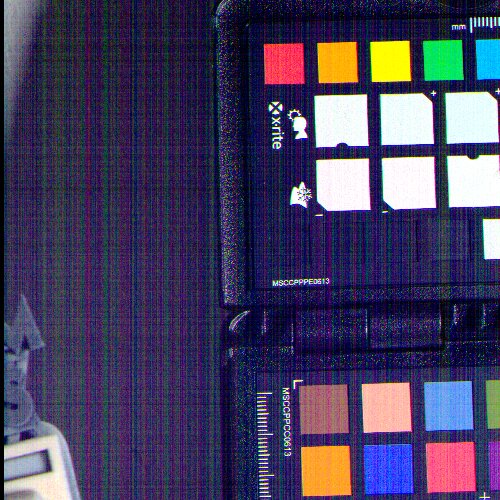
\includegraphics[height=5cm]{images/10ms+4-totally-raw-crop}
\end{center}

\begin{center}
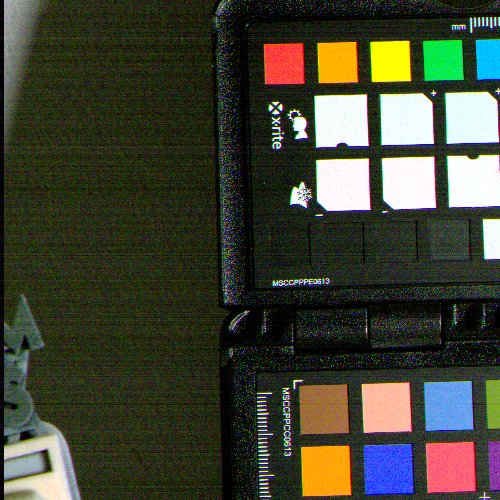
\includegraphics[height=5cm]{images/10ms+4-no-blackcol-crop}
\end{center}

- Left: after dark frame, dark current and static offsets from black reference columns.\\
- Right: after dark frame, dark current and black reference columns correction, without removing the fixed frequency component.\\

 \begin{center}
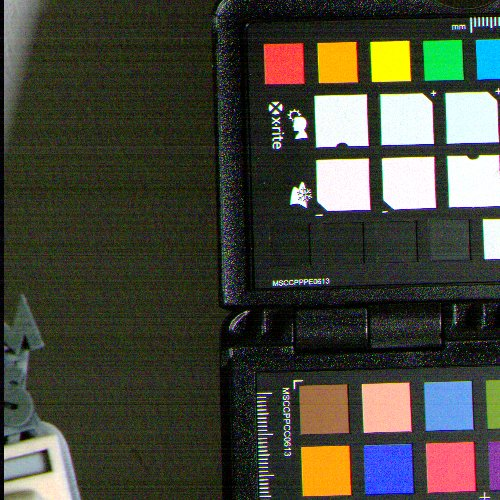
\includegraphics[height=5cm]{images/10ms+4-no-blackcol-rn-crop}
\end{center}

\begin{center}
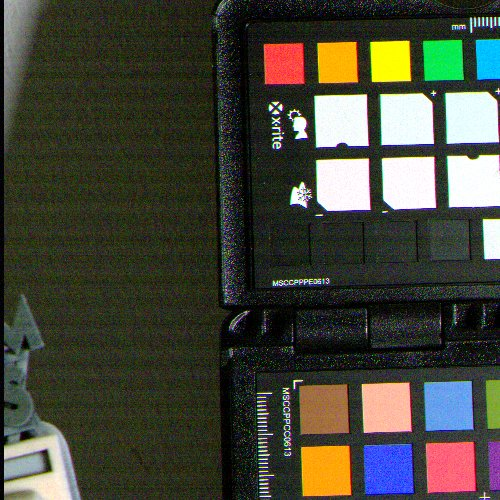
\includegraphics[height=5cm]{images/10ms+4-no-blackcol-ff-crop}
\end{center}

- Left: after dark frame, dark current and black reference columns correction.\\
- Right: after row noise reduction \importantKeyword{--fixrn} \\

\begin{center}
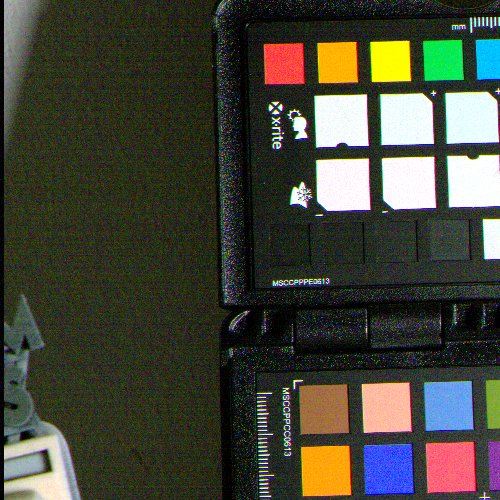
\includegraphics[height=5cm]{images/10ms+4-crop}
\end{center}

\begin{center}
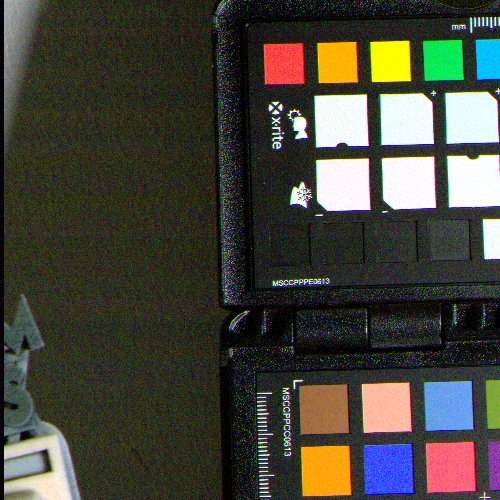
\includegraphics[height=5cm]{images/10ms+4-fixrn-crop}
\end{center}

- Left: \importantKeyword{--rnfilter=1} \\
- Right: \importantKeyword{--rnfilter=2} \\

\begin{center}
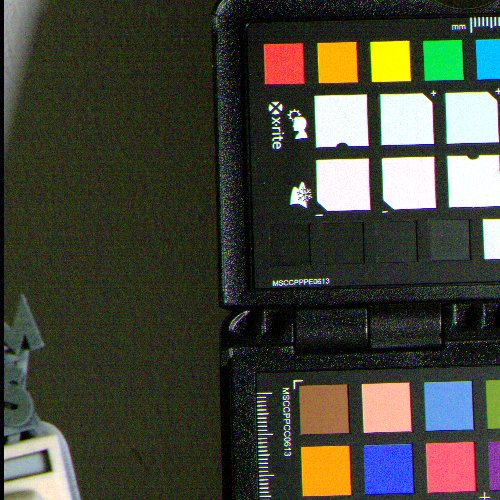
\includegraphics[height=5cm]{images/10ms+4-rnfilter1-crop}
\end{center}

\begin{center}
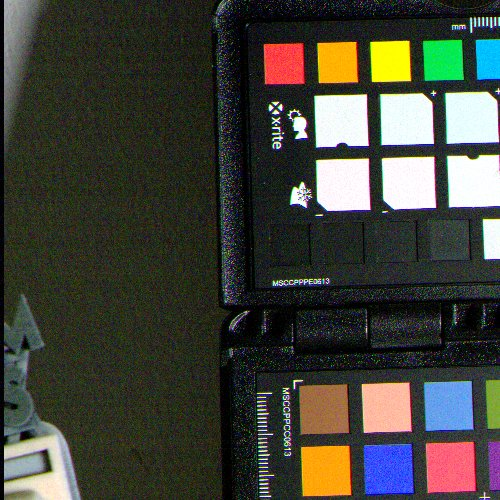
\includegraphics[height=5cm]{images/10ms+4-rnfilter2-crop}
\end{center}

Algorithm internals for \importantKeyword{--fixrn}

- Left: filtered image (vertical blur using a bilateral filter)\\
- Right: noise image, revealing row noise. Black regions are from edges that were masked.\\ 

\begin{center}
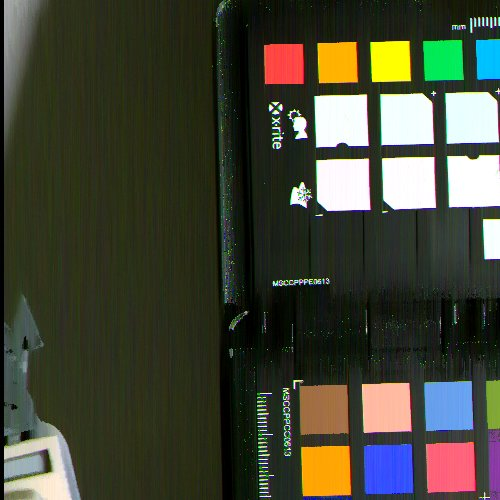
\includegraphics[height=5cm]{images/10ms+4-fixrn-dbg-denoised-crop}
\end{center}

\begin{center}

\includegraphics[height=5cm]{images/10ms+4-fixrn-dbg-noise-crop}
\end{center}

\textbf{Downsized images}\\

Corrected with dark frame and dark current only:\\
 
\begin{center}
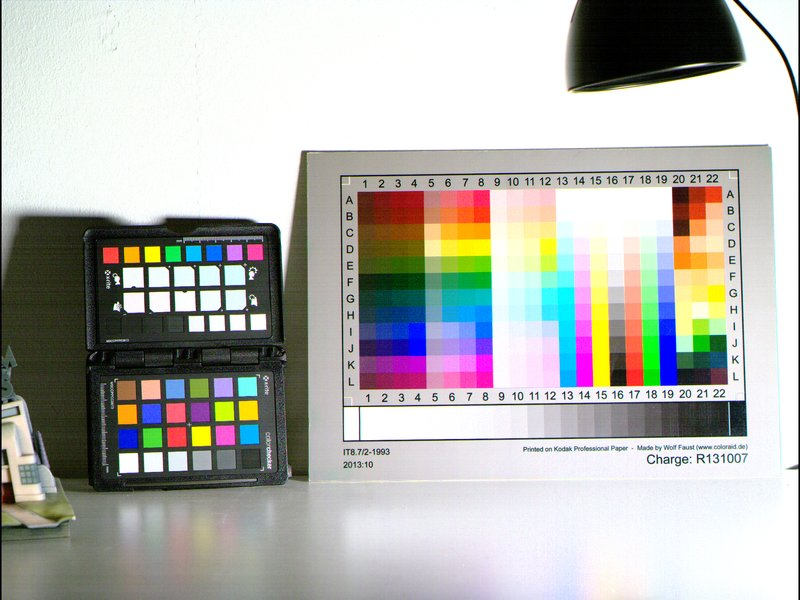
\includegraphics[height=5cm]{images/10ms+4-no-blackcol-small}
\end{center}

Also corrected with black columns: 

\begin{center}
%\includegraphics[height=5cm]{images/10ms+4-smallp}
\end{center}

Also corrected with \importantKeyword{--fixrn} 

\begin{center}
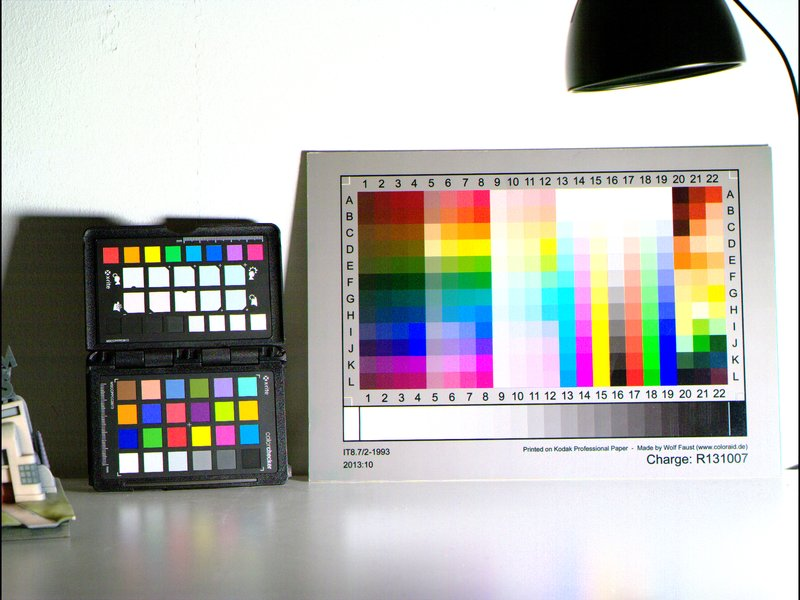
\includegraphics[height=5cm]{images/10ms+4-fixrn-small}
\end{center}

Corrected with \importantKeyword{--rnfilter=2}

\begin{center}
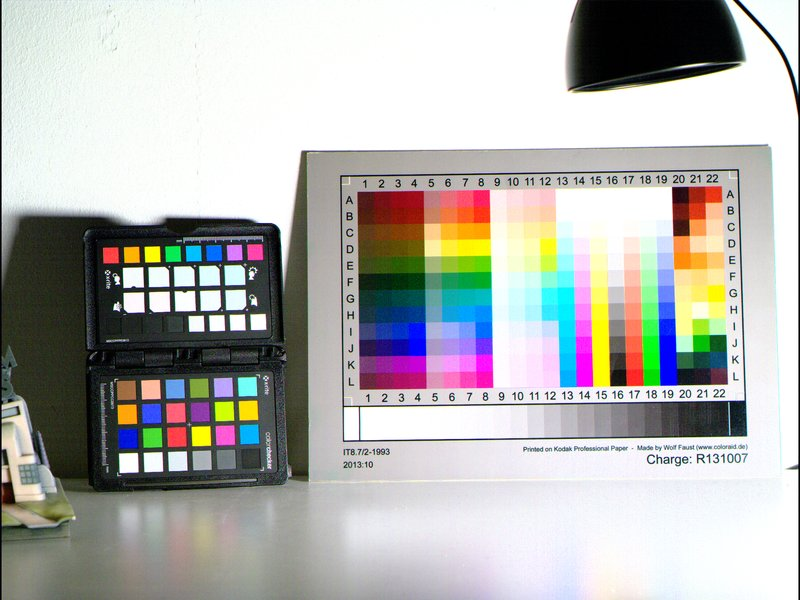
\includegraphics[height=5cm]{images/10ms+4-rnfilter2-small}
\end{center}

Larger images (half-res): \\

- 10ms+4-no-blackcol.jpg - \href{http://files.apertus.org/AXIOM-Beta/snapshots/pattern-noise/10ms+4-no-blackcol.jpg}{http://files.apertus.org/AXIOM-Beta/snapshots/pattern-noise/10ms+4-no-blackcol.jpg}\\
- 10ms+4.jpg - \href{http://files.apertus.org/AXIOM-Beta/snapshots/pattern-noise/10ms+4.jpg}{http://files.apertus.org/AXIOM-Beta/snapshots/pattern-noise/10ms+4.jpg}\\
- 10ms+4-fixrn.jpg - \href{http://files.apertus.org/AXIOM-Beta/snapshots/pattern-noise/10ms+4-fixrn.jpg}{http://files.apertus.org/AXIOM-Beta/snapshots/pattern-noise/10ms+4-fixrn.jpg}\\
- 10ms+4-rnfilter2.jpg - \href{http://files.apertus.org/AXIOM-Beta/snapshots/pattern-noise/10ms+4-rnfilter2.jpg}{http://files.apertus.org/AXIOM-Beta/snapshots/pattern-noise/10ms+4-rnfilter2.jpg} \\

\href{http://files.apertus.org/AXIOM-Beta/snapshots/pattern-noise/10ms+4-no-blackcol.jpg}{10ms+4-no-blackcol.jpg}\\
\href{http://files.apertus.org/AXIOM-Beta/snapshots/pattern-noise/10ms+4.jpg}{10ms+4.jpg}\\
\href{http://files.apertus.org/AXIOM-Beta/snapshots/pattern-noise/10ms+4-fixrn.jpg}{Final10ms+4-fixrn.jpg}\\
\href{http://files.apertus.org/AXIOM-Beta/snapshots/pattern-noise/10ms+4-rnfilter2.jpg}{10ms+4-rnfilter2.jpg}\\

All files used for this test, including scripts, calibration frames and uncompressed images, can be found here: \href{http://files.apertus.org/AXIOM-Beta/snapshots/pattern-noise/}{here}.\\

\href{http://files.apertus.org/AXIOM-Beta/snapshots/pattern-noise/10ms.raw12Raw12}{image: 10ms.raw12}\\
\href{http://files.apertus.org/AXIOM-Beta/snapshots/pattern-noise/darkframe-x1.pgm}{Calibration frames: darkframe-x1.pgm} and \href{http://files.apertus.org/AXIOM-Beta/snapshots/pattern-noise/dcnuframe-x1.pgm}{dcnuframe-x1.pgm}\\
\href{http://files.apertus.org/AXIOM-Beta/snapshots/pattern-noise/10ms.DNG}Final image (--rnfilter=2): {10ms.DNG}\\
\href{http://files.apertus.org/AXIOM-Beta/snapshots/pattern-noise/fpntest.sh}{Testing script: fpntest.sh}\\
\href{http://files.apertus.org/AXIOM-Beta/snapshots/pattern-noise/fpntest.log}{Script output: fpntest.log}\\






\subsection{Matrix Color Conversion} %See also mat4_conf.sh

Each color channel is going through 4 stages that each look like this: (I+A)*E+O 

\begin{lstlisting}[language=bash,morekeywords=$,keywordstyle=\bfseries,frame=none,xleftmargin=.25in,belowskip=2em, aboveskip=2em]
    I = input (25bit unsigned)
    A = adjustment (30bit signed)
    E = matrix coefficient (18bit signed)
    O = offset (48bit signed)
\end{lstlisting}

The four stages are connected together that the offset of stage N is the output of stage N-1. The offset of stage 1 is set in registers (32-35). The output of stage 4 is the final result.\\


For each channel that results in the following fomular: 

\consoleCommand{Ri = SUMj ((Ij + Aij) * Eij) + Oi} 

Which in other words mean the result of matrix \importantKeyword{Eij} multiplied with an input vector \importantKeyword{Ij + Aij} plus an offset vector \importantKeyword{Oi}.

Currently all registers (beside input/output) are shortened to 16bit signed (this could be changed easily) values so the matrix is currently limited to 1/256 of the possible accuracy (due to a 8bit shift of the output).\\

All input/output register are tested for over/underflow and clipped to 12 bit (this can also be disabled).\\ 

\textbf{Setting/Getting Registers: }\\

\consoleCommand{. ./hdmi.func # load functions} 

\consoleCommand{    mat\_reg 0 # Read value of register 0 = A0
    mat\_reg 0 1 # Sett value of register 0 (A0) to 1} 
    
4x4 matrix coefficients (A0, A1, A2, A3, B0, B1, B2, B3, B4, C0, C1, C2, C3, D0, D1, D2, D3) are mapped to addresses 0 - 15. In registers 16 - 31 there are adjustment values and from 32 - 35 there are 4 offset values.\\

Input format per default is (R, G1, G2, B).\\

All values of the 4x4 matrix can be set conveniently with this script:\\

\consoleCommand{./mat4\_conf.sh  A0 A1 A2 A3  B0 B1 B2 B3 B4  C0 C1 C2 C3  D0 D1 D2 D3    O1 O2 O3 O4}    
    
Where the last quadruple is optional, it defaults to 0.\\

An RGB 3x3 matrix can easily be extended to a 4x4 matrix by using the coefficient for green and offsets twice or better to half both of the green coefficients and use the same value for both greens twice. \\    
    
\begin{center}

\includegraphics[height=5cm]{images/Eqn5}
\end{center}
    
    
    
    
    
   

\subsubsection{mat4\_conf.sh}

To set the 4x4 color conversion matrix, you can use the mat4\_conf.sh script:\\

The default configuration: 

\consoleCommand{./mat4\_conf.sh  1 0 0 0  0 1 0 0  0 0 1 0  0 0 0 1  0 0 0 0 } 

\textbf{Note:} In current AXIOM Beta firmware the mat4 order is changed and the default matrix is: 

\consoleCommand{./mat4\_conf.sh 0.3 0.3 0.3 0.3  0 0 0 1  0 0.42 0.42 0  1 0 0 0} 

This will be changed to reflect the documentation again soon.\\

With the Blackmagic Video Assist (BMVA), a nicer matrix (ie better skin color, less greenish): 

\consoleCommand{./mat4\_conf.sh 0.3 0.3 0.3 0.3  0 0 0 1  0 0.3 0.3 0  1 0 0 0} 

This 4x4 conversion matrix is a very powerful tool and allows to do things like mixing color channels, reassigning channels, applying effects or doing white balancing.\\

TODO: order is blue, green, red! 

\begin{center}
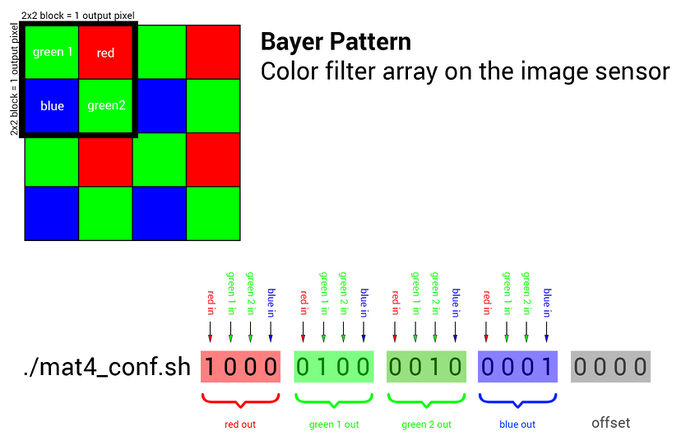
\includegraphics[height=5cm]{images/700px-Mat4-conf-illustration-01}
\end{center}

4x4 Matrix Examples:

\begin{lstlisting}[language=bash,morekeywords=$,keywordstyle=\bfseries,frame=none,xleftmargin=.25in,belowskip=2em, aboveskip=2em]
    ./mat4\_conf.sh  1 0 0 0  0 1 0 0  0 0 1 0  0 0 0 1    0 0 0 0   # unity matrix but not optimal as both green channels are processed separately
    ./mat4\_conf.sh  1 0 0 0  0 0.5 0.5 0  0 0.5 0.5 0  0 0 0 1    0 0 0 0   # the two green channels inside each 2x2 pixel block are averaged and output on both green pixels
    ./mat4\_conf.sh  0 0 0 1  0 1 0 0  0 0 1 0  1 0 0 0    0 0 0 0   # red and blue are swapped
    ./mat4\_conf.sh  1 0 0 0  0 1 0 0  0 0 1 0  0 0 0 1    0.5 0 0 0    # red 50% brigther
    ./mat4\_conf.sh  1 0 0 0  0 1 0 0  0 0 1 0  0 0 0 1.5    0 0 0 0    # blue multiplied with factor 1.5
    ./mat4\_conf.sh  .25 .25 .25 .25  .25 .25 .25 .25  .25 .25 .25 .25  .25 .25 .25 .25    0 0 0 0    # black/white
    ./mat4\_conf.sh  -1 0 0 0  0 -0.5 -0.5 0  0 -0.5 -0.5 0  0 0 0 -1    1 1 1 1    # negative
\end{lstlisting}






\subsection{CMV12000 PLR}

Some attempts to reverse engineer the PLR high dynamic range mode from CMV12000.\\ 

- 79: Number\_slopes: 1,2,3.\\
- 75-78: Exp\_kp1, Exp\_kp2: exposure times for highlights (same formula as Exp\_time)\\
- 106: Vtfl2, Vtfl3: knee point locations (range: 0-63; units: unknown) \\


\textbf{Register effects}.\\

I'll use an IT8 chart, exposed at 30 ms (normal exposure) and 100 ms (overexposed). A little dark in the lab today, but shouldn't be a big problem.\\

To analyze the images, I'll use octave 4.0, compiled with \href{http://marcelojoeng.blogspot.co.uk/2012/11/compile-octave-using-1632-bits-colour.html}{16-bit image support}. The scripts should run in Matlab as well, with minimal changes.\\

\subsubsection{Linear exposures}

\begin{center}
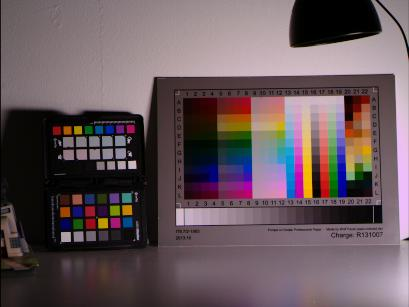
\includegraphics[height=5cm]{images/30ms-lin}
\end{center}

\begin{center}
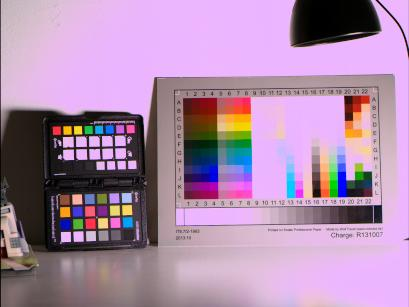
\includegraphics[height=5cm]{images/100ms-lin}
\end{center}

Let's check if the first image is really exposed to the right, in octave.  

\begin{lstlisting}[language=bash,morekeywords=$,keywordstyle=\bfseries,frame=none,xleftmargin=.25in,belowskip=2em, aboveskip=2em]
    a = read\_raw('30ms-lin.DNG');
    prctile(a(:),99) - 128        % note: black level is forced to 128 in raw2dng
    ans =  2269                   % clipping starts at about 2400-2500 above black
\end{lstlisting}

Let's check if the clipping point is, indeed, where I say: 

\begin{lstlisting}[language=bash,morekeywords=$,keywordstyle=\bfseries,frame=none,xleftmargin=.25in,belowskip=2em, aboveskip=2em]
    figure, hold on
    colors = 'rgcb';                                  % meaning: red, gren1, green2 (plotted as cyan), blue (raw data from Bayer channels)
    [g30,c30]   = sample_it8('30ms-lin.DNG', 0);      % read median RGGB swatch values from IT8 chart
    [g100,c100] = sample_it8('100ms-lin.DNG', 0);     % first output arg is grayscale, second is full color, each column is a Bayer channel
    for i = 1:4
      plot(c30(:,i), c100(:,i), ['.' colors(i)]);     % plot the 100ms image vs the 30ms one (extremely rough guess for response curve)
    end
\end{lstlisting}

\begin{center}
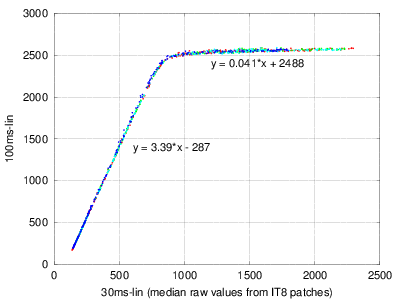
\includegraphics[height=5cm]{images/100ms-vs-30ms-lin}
\end{center}

- This approximates (but it's not equal to!) the response curve without PLR.\\
- This plot assumes the sensor response in the 30ms image (which was not overexposed) is linear (but it's probably not).\\
- The sensor doesn't clip very harshly to white (could be the PLR circuits kicking in with a very low exposure time? to be checked).\\

\subsubsection{2-segment PLR exposures}

Let's start with a 2-segment PLR exposure, 100ms/10ms, vtfl2=32. That means, Number\_slopes = 2, Exp\_time = 8072, Exp\_kp1 = 805, Vtfl=96. 

\begin{center}
\includegraphics[height=5cm]{images/100ms-10ms-32}
\end{center}

Although the image may look a little overexposed at first sight (because of the magenta cast), the raw levels seem to be alright: 

\begin{lstlisting}[language=bash,morekeywords=$,keywordstyle=\bfseries,frame=none,xleftmargin=.25in,belowskip=2em, aboveskip=2em]
    c = read\_raw('100ms-10ms-32.DNG');
    prctile(c(:),99)
    ans =  1957
\end{lstlisting}


Let's check our response curve approximation:

 \begin{lstlisting}[language=bash,morekeywords=$,keywordstyle=\bfseries,frame=none,xleftmargin=.25in,belowskip=2em, aboveskip=2em]
    [g100p,c100p] = sample\_it8('100ms-10ms-32.DNG', 0);
    figure, hold on
    for i = 1:4
      plot(c30(:,i), c100p(:,i), ['.' colors(i)]);
    end
\end{lstlisting}

\begin{center}
\includegraphics[height=5cm]{images/100-10-32-plr-vs-30ms-lin}
\end{center}

- The knee point isn't as sharp as in the datasheet.\\
- Its location is around 400 (todo: find the relationship between this and vtfl).\\
- The second exposure segment appears a little noisy .\\

\subsubsection{Changing Exp\_kp1}

Let's leave Vtfl constant and change exposure time for the second segment (0,1,5,10,20,35,50 ms). 

\begin{center}
\includegraphics[height=5cm]{images/100ms-0ms-32-tiny}
\end{center}

\begin{center}
\includegraphics[height=5cm]{images/100ms-1ms-32-tiny}
\end{center}

\begin{center}
\includegraphics[height=5cm]{images/100ms-5ms-32-tiny}
\end{center}

\begin{center}
\includegraphics[height=5cm]{images/100ms-10ms-32-tiny}
\end{center}

\begin{center}
\includegraphics[height=5cm]{images/100ms-20ms-32-tiny}
\end{center}

\begin{center}
\includegraphics[height=5cm]{images/100ms-35ms-32-tiny}
\end{center}

\begin{center}
\includegraphics[height=5cm]{images/100ms-50ms-32-tiny}
\end{center}

Commands for plotting the "response curve" approximations are left as an exercise to the reader. Result: 

\begin{center}
\includegraphics[height=5cm]{images/100-x-32-plr-vs-30ms-lin}
\end{center}

\subsubsection{Changing Vtfl}

Now let's leave exposure time constant (100ms/1ms) and change Vtfl (off,0,8,16,24,32,40,48,56,63): 

\begin{center}
\includegraphics[height=5cm]{images/100ms-1ms-00-tiny}
\end{center}

\begin{center}
\includegraphics[height=5cm]{images/100ms-1ms-0-tiny}
\end{center}

\begin{center}
\includegraphics[height=5cm]{images/100ms-1ms-8-tiny}
\end{center}

\begin{center}
\includegraphics[height=5cm]{images/100ms-1ms-16-tiny}
\end{center}

\begin{center}
\includegraphics[height=5cm]{images/100ms-1ms-24-tiny}
\end{center}

\begin{center}
\includegraphics[height=5cm]{images/100ms-1ms-32-tiny}
\end{center}

\begin{center}
\includegraphics[height=5cm]{images/100ms-1ms-40-tiny}
\end{center}

\begin{center}
\includegraphics[height=5cm]{images/100ms-1ms-48-tiny}
\end{center}

\begin{center}
\includegraphics[height=5cm]{images/100ms-1ms-56-tiny}
\end{center}

\begin{center}
\includegraphics[height=5cm]{images/100ms-1ms-63-tiny}
\end{center}

\begin{center}
\includegraphics[height=5cm]{images/100-1-x-plr-vs-30ms-lin}
\end{center}

\subsubsection{Changing Exp\_time}

Now let's leave \importantKeyword{Exp\_kp1} and \importantKeyword{Vtfl} constant (0ms/32) and change base exposure time (20,50,100,150 ms):\\

\begin{center}
\includegraphics[height=5cm]{images/x-0-32-plr-vs-30ms-lin}
\end{center}

- There is a noticeable light leak in the second segment, but it doesn't seem to change with base exposure time.\\
- Most of the noise in these curves seems static (correctable with calibration frames). \\

\subsubsection{Changing Exp\_kp2 and Vtfl3}

As expected, these settings do not seem to have any noticeable effect when \importantKeyword{num\_slopes = 2}. 


\subsubsection{Mathematical models}

\textbf{First models of the response curve for 2-segment PLR exposures.}

Let's go back to the scenario with constant Vtfl and variable exposure. 

\begin{center}
\includegraphics[height=5cm]{images/100-x-32-plr-vs-30ms-lin}
\end{center}

Notice the knee point appears to move to the right with higher Exp\_kp1 values. Why would this happen?\\

If we assume the knee point threshold (Vtfl2) is only monitored while we still have time to fully expose the second segment (Exp\_kp1), we can imagine a model of the PLR exposure that looks like this:\\

\begin{lstlisting}[language=bash,morekeywords=$,keywordstyle=\bfseries,frame=none,xleftmargin=.25in,belowskip=2em, aboveskip=2em]
    function y = plr\_model_0(x, exp\_time, vtfl\_thr, exp\_kp1)
       % regular exposure time
       y = x .* ex\p_time;
       
       % time needed to reach the Vtfl threshold (lower input levels => longer times)
       t\_reach\_vtfl = vtfl\_thr ./ x;
       
       % which pixels reach vtfl?
       % assume this threshold is only monitored while we still have time
       % to fully perform the exp\_kp1 (that is, before exp_time - exp\_kp1)
       reached\_vtfl = t\_reach\_vtfl < exp\_time - exp\_kp1;
       
       % how the exposure behaves in the highlights
       y\_highlight = vtfl\_thr + x .* exp\_kp1;
       
       % copy highlight values only for those pixels that reached Vtfl
       y(reached\_vtfl) = y\_highlight(reached\_vtfl);
    end
\end{lstlisting}

Let's see how it compares to our real data. \\

\begin{center}
\includegraphics[height=5cm]{images/100-x-32-plr-vs-30ms-lin-model0}
\end{center}

Notice the slopes of the second segment seem to be higher in the real data, compared to our model, as if the real exposure time would be a little higher.

Since the slope at \importantKeyword{exp\_kp1=0} doesn't depend on total exposure time, let's assume there is some sort of exposure leak - that is, the actual exposure time is \importantKeyword{exp\_kp1} + some constant (called \importantKeyword{exp\_leak} ). 


\begin{lstlisting}[language=bash,morekeywords=$,keywordstyle=\bfseries,frame=none,xleftmargin=.25in,belowskip=2em, aboveskip=2em]
    function y = plr\_model\_1(x, exp\_time, vtfl\_thr, exp\_kp1, exp\_leak)
      
       [ ... ]  
      
       % how the exposure behaves in the highlights
       y\_highlight = vtfl\_thr + x .* (exp\_kp1 + exp\_leak);
      
       [ ... ]  
      
    end
\end{lstlisting}

\begin{center}
\includegraphics[height=5cm]{images/100-x-32-plr-vs-30ms-lin-model1}
\end{center}

Tuning parameters (trial and error): \importantKeyword{vtfl\_thr = 850}, \importantKeyword{exp\_leak = 2.5ms}.\\

Black level 128 (after subtracting black reference columns, dark frame and dark current nonuniformity). Reference frames obtained from fitting 256 dark frames taken at exposures from 1 to 64 ms, in 1 ms increments, 4 images at each exposure, with raw2dng --swap-lines --calc-dcnuframe *x1*.raw12.\\

This model appears to explain the actual response curves pretty well, but there's still room for improvement. \\

\textit{At this point, I would try to find some real response curves and reduce the noise of the test images by averaging multiple frames, then repeat the experiment. This will take a while.}\\

After averaging 50 frames at each setting, the noise in the curve remained the same, so it must be systematic error (correctable with some sort of calibration frame).\\

Finding response curves from bracketed images is difficult - we can't just scale exposure times hoping we'll get the same curve. We will need a dimmable light source with no ambient light (or some dedicated calibration hardware).\\


To be continued. 








\subsection{CMV12000 Response Curves}

\textbf{Identifying response curves on the CMV12000 sensor }\\

We would like the data coming from the sensor to be linear (that is, proportional to the number of photons received). Plus some constant offset.\\

Is it already linear, or do we have to adjust it?\\

This sensor has a high dynamic range mode called PLR (piecewise linear response). In this mode, the sensor response is highly nonlinear (configurable, but the output is not exactly piecewise linear, so we still have to identify the curves). Details about this mode on the PLR page.\\

Here we'll focus on identifying the response curves.\\

eg: input range where the linear sensor response, and use that range to correct nonlinearities that occur outside this range (for example, with underexposure, overexposure, or by comparing a PLR mode with a regular exposure mode). This can be good enough for initial tests, but it has a major problem. \\

Suppose we have a sensor with this response: \importantKeyword{y = (t*x)\^2 }(where t is exposure time, x is radiance, x*t is the number of photons captured, and y is the sensor output value, all in arbitrary units). Let's expose two synthetic images from it, in octave: 

\begin{lstlisting}[language=bash,morekeywords=$,keywordstyle=\bfseries,frame=none,xleftmargin=.25in,belowskip=2em, aboveskip=2em]
    x = linspace(0, 1, 1000);             % synthetic "image" with range from 0 to 1 (black to white)
    a = x.^2;                             % "expose" the image for 1 time unit
    b = (3*x).^2;                         % "expose" the image for 3 time units
    subplot(131), plot(x, a, x, b)        % plot the sensor responses vs input signal (radiance)
    subplot(132), plot(a, b);             % plot the second image, under the assumption that first one might be linear
    subplot(133), plot(log2(a), log2(b)); % also try a logarithmic plot
    hold on, plot(log2(a),log2(3*a),'k'); % expected response for the logarithmic plot
\end{lstlisting}

\begin{center}
\includegraphics[height=5cm]{images/naive}
\end{center}

Our simulated sensor has obviously nonlinear sensor response, yet comparing two images suggest its output might be actually linear.\\

However, the log plot indicates there may be a problem, so this type of nonlinearity is not really 100% hidden. One could also think the exposure controls on the sensor were not accurate (in this case, you would also get an offset between the two curves, so it's easy to mistake these two situations).\\

This nonlinearity was pretty obvious, but subtler variations may be much more difficult to spot, so we should really find a way to recover the true response curve. Without a photon counter, that is. \\

\textbf{Test data}\\

Bracketed image of the grayscale line from an IT8 chart, 1...100ms in 1ms increments, exposure sequence executed 100 times, images at identical settings averaged. 

\begin{center}
%\includegraphics[height=5cm]{images/it8-grayscale}
\end{center}

\textbf{Existing algorithms}\\

- Review: Best algorithms for HDR image generation. A study of performance bounds. \href{https://hal.archives-ouvertes.fr/file/index/docid/733853/filename/best_hdr_algo_hal.pdf}{Ref.}\\
- Debevec97 \href{http://www.pauldebevec.com/Research/HDR/debevec-siggraph97.pdf}{Ref 01.} k\href{http://pages.cs.wisc.edu/~csverma/CS766_09/HDRI/hdr.html}{Ref 02}, implemented in mkhdr \href{http://duikerresearch.com/mkhdr-archive/}{Ref 03}.\\
- Robertson02 \href{http://pages.cs.wisc.edu/~lizhang/courses/cs766-2008f/projects/hdr/Robertson2003ETA.pdf}{Ref 01}, implemented in pfshdrcalibrate \href{http://resources.mpi-inf.mpg.de/hdr/calibration/pfs.html}{Ref 02}.\\
- ArgyllCMS, shaper+matrix algorithm\\
- other algorithms that we can try? \\


\subsubsection{Debevec97 results}

\textbf{Robertson02 results}

\begin{center}
\includegraphics[height=5cm]{images/response-curve-pfs}
\end{center}

These curves seem to indicate that our black level may be a little too high. Figure out why. \\

Scripts, logs: \href{http://files.apertus.org/AXIOM-Beta/snapshots/response-curves/pfs/}{http://files.apertus.org/AXIOM-Beta/snapshots/response-curves/pfs/}\\

\paragraph{ArgyllCMS shaper+matrix results}

WIP, source code - \href{https://github.com/apertus-open-source-cinema/misc-tools-utilities/commit/155be5e8cac9c7d158b8cf1a3055c833c9eab9a9}{https://github.com/apertus-open-source-cinema/misc-tools-utilities/commit/155be5e8cac9c7d158b8cf1a3055c833c9eab9a9}.\\

Q: can this be used on bracketed images?\\


\subsubsection{Custom algorithms}

\paragraph{Median vs exposure}\mbox{}\\

This assumes the exposure setting from the sensor is accurate, so the input signal that will be digitzed is proportional to number of photons (scene radiance multiplied by exposure time.\\

Unfortunately, this method delivered inconsistent results (two experiments resulted in two different curves -

\begin{center}
\includegraphics[height=5cm]{images/curve-new}
\end{center}

\begin{center}
\includegraphics[height=5cm]{images/curve-old}
\end{center}


\subsubsection{Black Hole anomaly}

Here's an example showing how much the exposure setting can be trusted. Crop taken from a bracketed exposure (1,2,5,10,20,30 ms) repeated 700 times and averaged. Image from the figure is from the 30ms exposure.\\ 

\begin{center}
\includegraphics[height=5cm]{images/blackhole}
\end{center}

That's right - when exposure time increases, very dark pixels become even darker.\\

Also note the black level, after correcting the image with dark frames and black reference columns, is set to 128 (the entire image is adjusted by adding a constant, so the black reference columns reach this value). The pixels showing this anomaly are below this black level. There is detail in the image, even in a single (non-averaged) exposure, but for some unknown reason, it ends up below the black level.\\

This behavior cannot be reproduced on dark frames though, so probably (unconfirmed hypothesis) the black level goes down (not sure if globally or locally) when the image content gets brighter. The detail in the dark area on the test image looks normal (not reversed), so probably the total number of photons captured is the variable we should account for? \\


\subsubsection{Matching per-pixel curves}

This algorithm is roughly inspired from Robertson02, but without any solid mathematical background; only with the hope that it will converge to a good solution.\\

1. Initial guess:\\

- Plot per-pixel response curves on a graph, trusting exposure control on the sensor for accuracy.\\
- For each sensor output value, let's say from 16 to 2048 in 0.25-stop increments, compute the median exposure required to get that output.\\
- Shift each curve horizontally, in log space, to match the median exposure.\\
- Repeat until convergence.\\
 
1. Refinement:\\

- Assume each pixel curve may be shifted by a constant offset vertically.\\
- Repeat the same algorithm used for initial guess, but also shift the curves vertically, in linear space, by a constant offset.\\
- Assume the average shift value is 0 (the algorithm may converge to a wrong solution without this constraint).\\

Problems:\\

- You can't operate on too many pixel curves at once (it can get slow and memory-intensive).\\
- There's no proof on whether it will converge, and if yes, how accurate the solution will be (but we can try it on synthetic data).\\ 

Example (only a single line from the test images was used): \\

Initial guess:\\

\begin{center}
\includegraphics[height=5cm]{images/response-curve-test-init}
\end{center}

Second guess:\\

\begin{center}
\includegraphics[height=5cm]{images/response-curve-test}
\end{center}

\textbf{Note:} The response looks a bit different from Robertson02. Who is right?\\




\subsubsection{Direct per-pixel curves}

Storing response curves for each pixel would be really expensive in terms of storage (memory), but may be worth trying.\\

Test data: bracketed exposures at 1,2,5,10,20,30 ms. 700-frame average for each exposure (total 4200 images, captured overnight). This would reduce dynamic noise by log2(sqrt(700)) = 4.7 stops, so the static variations should be reasonably clean.\\

Since the test image was not perfectly uniform (since we didn't actually shoot a flat field frame), we probably won't be able to find out the PRNU. \\



\subsubsection{WIP}

\paragraph{Curves from grayscale IT8 reference data}\mbox{}\\

Response curves can be also estimated from the IT8 reference data, which was (hopefully) measured with much better accuracy than what we can achieve with our current setup.\\

Advantage:\\

- We have some absolute reference data.\\
- We can get a quick estimation of some part of the curve from a single image.\\ 

Problems:\\

- In our setup, the illumination is nonuniform.\\
- Tthe dynamic range of the IT8 chart is not very high (7.33 stops on the bottom gray scale).\\
- Few data points (because, without a matrix, we can only use grayscale swatches; on the good side, these few data points are not very noisy).\\ 

Solutions/workarounds:\\

- We can account for the nonuniform illumination by checking the brightness levels at the edges of the chart (light gray); it's not very exact, just better than nothing.\\
- To cover the entire dynamic range, we can use bracketed images, but this is not perfect - the image levels appear to vary with number of photons, see the \textbf{Black Hole anomaly}.\\
- We may be able to use the curve matching algorithm to account for these unwanted variations with exposure time.\\

 
\paragraph{Correcting for nonuniform illumination}\mbox{}\\

Sampling data from the edge of the chart (left) lets us correct for nonuniform illumination: one can either adjust the chart itself (right), or the reference data (preferred).\\

\begin{center}
\includegraphics[height=5cm]{images/it8_lum_sampling_areas}
\end{center}

\begin{center}
\includegraphics[height=5cm]{images/it8_lum_correction}
\end{center}

See also:\\

\begin{center}
\includegraphics[height=5cm]{images/it8_lum_correction_3d}
\end{center}

\begin{center}
\includegraphics[height=5cm]{images/it8_lum_correction_2d}
\end{center}

Why it's better to adjust the reference data instead of chart pixels?\\

- Black level in our setup is uncertain.\\
- The chart borders are fairly bright, so the measurements of border brightness are not really influenced by small black level variations.\\
- Adjusting the image must be done in log space, so we must operate on linearized data.\\
- If the black level is uncertain, the adjusted dark swatches will have large errors.\\
- If the response curve is not linear (and not known), adjusting the data under the assumption of linearity will introduce extra errors.\\
- On the other hand, reference IT8 data is already in linear XYZ space, so adjusting it will not introduce extra errors (other than our less-than-accurate measurements).\\
- The measurement errors can be hopefully solved with an iterative procedure (anyone able to prove it?).\\ 

Plotting raw data vs reference values on IT8 gray swatches gives:\\

\begin{center}
\includegraphics[height=5cm]{images/it8_lum_check}
\end{center}

In the left figure, the two grayscale lines from the IT8 chart diverge because of nonuniform illumination. After adjusting the reference data, the match is much better, though it's still not perfect (because we can't really measure the nonuniform illumination in the chart, other than by including it in the model when performing the color profiling step).\\

\paragraph{Iterative procedure for estimating the response curve in the presence of nonuniform illumination}\mbox{}\\

- Initial estimation of response curve, from noisy data (because of nonuniform illumination).\\
- Adjust the reference data from brightness on chart borders (use griddata to interpolate).\\
- Estimate the response curve again, this time from much cleaner data.\\
- Repeat steps 2-3 until convergence.\\ 

Unfortunately, this is not going to solve the mismatch between the two scales. Better get some properly illuminated charts :) 




\section{Associated Use-cases}
\subsection{Configuration for Photography}

\section{Hardware}
\subsection{PCB Stack Layout}
\subsubsection{Shields}
\subsubsection{Plugin Modules}
\subsubsection{EEPROM}
\subsection{PCB Revision Links}
\subsection{Power Supply}
\subsubsection{AC Power Supply}
\subsubsection{DC Power Supply}
\subsubsection{Active Battery Mount}
\subsection{Enclosure}
\subsubsection{Skeleton}
\subsubsection{Simple Enclosure}
\subsubsection{Transparent Acrylic Enclosure}
\subsection{Optical Information}
\subsubsection{Lens Mount}
\subsubsection{Lens Mount Overviews}
\subsubsection{Infra Red / Ultra Violet Cut-off Filter}
\subsubsection{Optical Low-pass Filter (OLPF)}

\section{Support}
\subsection{Contact Details and Communication Channels}
\subsection{Regional Communities}
\subsection{Useful Links}



%\\Test


\begin{lstlisting}[breaklines=true, breakatwhitespace=true]
    1: lo: <LOOPBACK,UP,LOWER_UP> mtu 65536 qdisc noqueue state UNKNOWN group default 
        link/loopback 00:00:00:00:00:00 brd 00:00:00:00:00:00
        inet 127.0.0.1/8 scope host lo
           valid_lft forever preferred_lft forever
        inet6 ::1/128 scope host 
           valid_lft forever preferred_lft forever
    2: eth0: <BROADCAST,MULTICAST,UP,LOWER_UP> mtu 1500 qdisc pfifo_fast state UP group default qlen 1000
        link/ether 00:0a:35:00:01:26 brd ff:ff:ff:ff:ff:ff
        inet 192.168.0.9/24 brd 192.168.0.255 scope global dynamic eth0
           valid_lft 172739sec preferred_lft 172739sec
        inet6 fe80::20a:35ff:fe00:126/64 scope link 
           valid_lft forever preferred_lft forever
\end{lstlisting}


\begin{lstlisting}
    cd ~/.ssh/
    cp authorized_keys authorized_keys.orig
\end{lstlisting}


ghgffghfg

\end{document}
